%% LyX 2.2.1 created this file.  For more info, see http://www.lyx.org/.
%% Do not edit unless you really know what you are doing.
\documentclass{article}\usepackage[]{graphicx}\usepackage[]{color}
%% maxwidth is the original width if it is less than linewidth
%% otherwise use linewidth (to make sure the graphics do not exceed the margin)
\makeatletter
\def\maxwidth{ %
  \ifdim\Gin@nat@width>\linewidth
    \linewidth
  \else
    \Gin@nat@width
  \fi
}
\makeatother

\definecolor{fgcolor}{rgb}{0.345, 0.345, 0.345}
\newcommand{\hlnum}[1]{\textcolor[rgb]{0.686,0.059,0.569}{#1}}%
\newcommand{\hlstr}[1]{\textcolor[rgb]{0.192,0.494,0.8}{#1}}%
\newcommand{\hlcom}[1]{\textcolor[rgb]{0.678,0.584,0.686}{\textit{#1}}}%
\newcommand{\hlopt}[1]{\textcolor[rgb]{0,0,0}{#1}}%
\newcommand{\hlstd}[1]{\textcolor[rgb]{0.345,0.345,0.345}{#1}}%
\newcommand{\hlkwa}[1]{\textcolor[rgb]{0.161,0.373,0.58}{\textbf{#1}}}%
\newcommand{\hlkwb}[1]{\textcolor[rgb]{0.69,0.353,0.396}{#1}}%
\newcommand{\hlkwc}[1]{\textcolor[rgb]{0.333,0.667,0.333}{#1}}%
\newcommand{\hlkwd}[1]{\textcolor[rgb]{0.737,0.353,0.396}{\textbf{#1}}}%
\let\hlipl\hlkwb

\usepackage{framed}
\makeatletter
\newenvironment{kframe}{%
 \def\at@end@of@kframe{}%
 \ifinner\ifhmode%
  \def\at@end@of@kframe{\end{minipage}}%
  \begin{minipage}{\columnwidth}%
 \fi\fi%
 \def\FrameCommand##1{\hskip\@totalleftmargin \hskip-\fboxsep
 \colorbox{shadecolor}{##1}\hskip-\fboxsep
     % There is no \\@totalrightmargin, so:
     \hskip-\linewidth \hskip-\@totalleftmargin \hskip\columnwidth}%
 \MakeFramed {\advance\hsize-\width
   \@totalleftmargin\z@ \linewidth\hsize
   \@setminipage}}%
 {\par\unskip\endMakeFramed%
 \at@end@of@kframe}
\makeatother

\definecolor{shadecolor}{rgb}{.97, .97, .97}
\definecolor{messagecolor}{rgb}{0, 0, 0}
\definecolor{warningcolor}{rgb}{1, 0, 1}
\definecolor{errorcolor}{rgb}{1, 0, 0}
\newenvironment{knitrout}{}{} % an empty environment to be redefined in TeX

\usepackage{alltt}
\usepackage[sc]{mathpazo}
\usepackage[T1]{fontenc}
\usepackage{geometry}
\geometry{verbose,tmargin=2.5cm,bmargin=2.5cm,lmargin=2.5cm,rmargin=2.5cm}
\setcounter{secnumdepth}{2}
\setcounter{tocdepth}{2}
\usepackage{url}
\usepackage[unicode=true,pdfusetitle,
 bookmarks=true,bookmarksnumbered=true,bookmarksopen=true,bookmarksopenlevel=2,
 breaklinks=false,pdfborder={0 0 1},backref=false,colorlinks=false]
 {hyperref}
\hypersetup{
 pdfstartview={XYZ null null 1}}
\usepackage{breakurl}
\IfFileExists{upquote.sty}{\usepackage{upquote}}{}
\begin{document}



\title{THE TAG LOCATION PROBLEM}
\label{chapter2}
\author{Michael D. Sumner}
\maketitle

\end document
This chapter discusses problems faced with tracking data that concern
the estimation of location and provides a flexible software
environment for exploring data and applying solutions. Examples are
used to illustrate the variety of problems and some of the limitations
of the traditional techniques by which tracking data are analysed. The
\pkg{trip} package is a dedicated suite of tools developed by the
author in the software language \proglang{R}. This package integrates
data handling and analytical techniques for track data with broader
GIS and spatial data tools. This makes track data handling tools
easily available, even for those without strong programming
skills. The chapter concludes by extending the concerns regarding
the limitations of traditional techniques to methods for deriving
locations from raw data.

% First we discuss the goals of location estimation for animal tracking
% and outline the problems involved even in ideal conditions. I discuss
% the additional problems encountered in practice, and the problems of
% imperfect data collection and logistical difficulties.

This chapter is not intended to be a critique of modern methods of
dealing with tracking data, but introduces the variety of issues
encountered and tools for applying them.  Simple-to-use tools for
handling spatial and temporal data are still rare and some of the
problems encountered cause difficulties for researchers before they
have an opportunity to explore sophisticated methods.  The aim here is
to illustrate some classical techniques within a software toolkit that
provides better control over the details of analysis tools for those
without advanced programming skills. Later chapters present solutions
for the remaining problems.  Work by \cite{patterson2008state} and
\cite{breedthesis} provide a more critical review of recent methods.

%% Chapter2 - ensure that AIMs are specified up front:
Aims of this chapter:

\begin{enumerate}
\item{To introduce existing problems in tracking analyses presented
    with examples of classical techniques. }
\item{To illustrate the complexity of problems and areas that require
    more sophisticated solutions than traditional techniques. The
    problems presented here illustrate the need for solutions that
    come later in the thesis.}
\item{To present a flexible and readily customized software package as
    a framework for classical analyses and starting point for more
    sophisticated analyses.}
\item{To explain the compromises that are often made with regard to
    data representation and storage, as dictated by traditional
    systems, rather than an expressive model of the problem
    represented by the spatial and temporal data.  }
\item{To encourage the use of techniques for automatic data
    validation, spatial and temporal data storage and integration with
    database and GIS technologies.}
\end{enumerate}

%To explain the compromises that are often made in terms of data
%storage and computation, rather than in terms of the modelling
%problems presented by spatial and temporal data.

\section{\proglang{R} and the \pkg{trip} package}

The software package \pkg{trip} developed with this chapter provides
an integrated system for data validation and a development framework
for track analyses. This can be used as a launching point for further
analysis such as validating input to Bayesian methods, or filtering
for state-space models \citep{patterson2010using}. As an extension of
the \proglang{R} environment, \pkg{trip} also provides integration
with tools for data access and output, integration with GIS and other
data systems, and metadata for projections and coordinate systems. The
\pkg{trip} package ties together numerous tracking analysis
techniques, which previously were only available though a wide variety
of disparate tools, each having various requirements and limitations.

         % The
% \pkg{trip} package was developed because not everything required by
% tracking analysis was available in one place, with many disparate
% tools having very different requirements and other limitations.

The \pkg{trip} package was developed within the freely available
software platform \proglang{R}, a statistical programming environment
consisting of a vast community of contributing developers and users
\citep{R}. \proglang{R} is organized into modules known as
\emph{packages} which provide the functionality of the language, and
also the mechanism by which it is extended\footnote{See
  \url{http://en.wikipedia.org/wiki/Package_Development_Process}.}. New
packages are created using the same tools by which R itself is built
and can be contributed to a public repository such as the
Comprehensive R Archive Network (\texttt{CRAN}\footnote{See
  \url{http://en.wikipedia.org/wiki/Software_repository}.}). The
repository system for contributed packages is one of the great
strengths of \proglang{R} and is part of the reason for its ease of
use and subsequent popularity. The spatial and temporal capabilities
of \proglang{R} are advanced, including strong integration with other
technologies such as databases, GIS software and the wide variety of
spatial and other complex data formats.

The data coercion paradigm in \proglang{R} is very powerful, allowing
rather different packages to share data with tight integration. There
are some fundamental data representations required for spatial
analysis and careful organization is needed to provide coercions
between different types to get all the tools to work together.  The
spatial infrastructure used to create the \pkg{trip} package is
described with examples of using the software in Section
\ref{sec:tripdemo}.


%Chapter2 - ensure that AIMs are specified up front:
% 1. aim to introduce what is to come later in thesis, in terms of
% existing problems and what can and cannot be done
% 2. trip as a framework for classical analyses and launchpad for more
% sophisticated (e.g. validated input to SS models)
%   - validation, launching point
%   - data integration, data access
%   - data output
%   - development framework
%   - projections/coordinate systems/ GIS


%  I explore
% some of the existing approaches and the types of studies with the aim
% of determining the general features of all, and how many of the
% existing techniques only partly solve some problems.  I talk about the
% under-use of GIS and projections in tracking applications, show how
% some difficulties could benefit from a wider understanding, and
% finally outline the need for an integrated approach to tracking
% problems with full models of both animal movement and data collection.

\section{Problems with location estimation}
\label{sec:locationproblems}
This section presents actual tag location estimates to illustrate
common problems associated with track data. The location data were
provided by System Argos, which is a worldwide satellite service that
provides location estimates from small mobile transmitters.

The first example is a sequence of Argos position estimates for a
single elephant seal in Figure~\ref{fig:RawArgos}. All raw estimates
provided are shown, with the longitude and latitude values transformed
to an equal-area projection and drawn connected as a line. While there
is obvious noise in the track, the general sequence of events is
clear: the seal leaves Macquarie Island, swimming predominantly
south-east to the Ross Sea where it spends several weeks, and then
returns via a similar path in reverse.




\begin{figure}
\begin{center}
\begin{knitrout}
\definecolor{shadecolor}{rgb}{0.969, 0.969, 0.969}\color{fgcolor}

{\centering 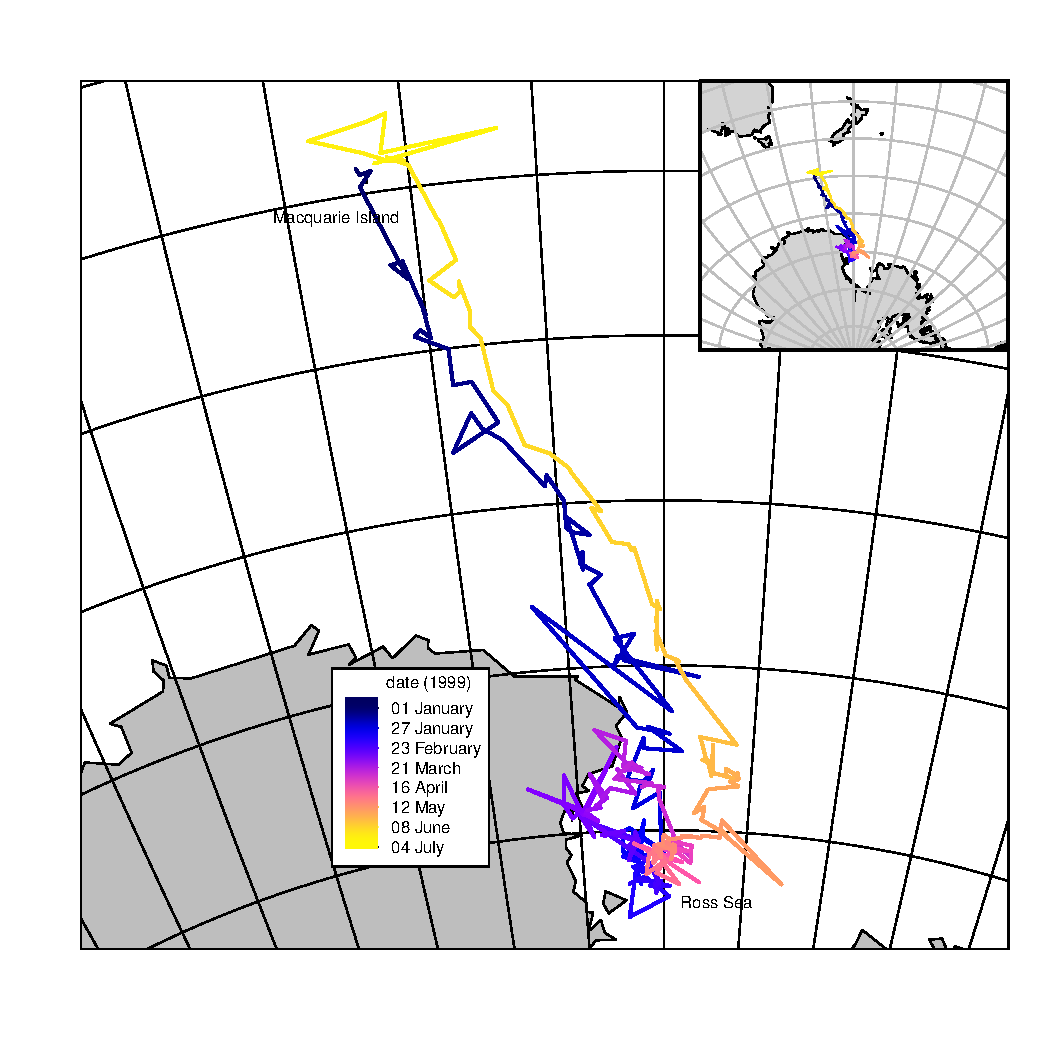
\includegraphics[width=\maxwidth]{figure/minimal-unnamed-chunk-2-1} 

}



\end{knitrout}
\end{center}
\caption{Raw Argos estimates for a Macquarie Island elephant seal.
  The line connecting the points is coloured from blue through purple
  to yellow in order relative to the time of each position. (Macquarie
  Island can just be seen in black beneath the third dark blue line
  segment). The outward and inward journeys are much faster than the
  journey throughout the Ross Sea, as shown by the colour scale
  change. A graticule is shown for scale, 5 degrees on the main plot,
  and 10 degrees on the inset. }
\label{fig:RawArgos}
\end{figure}

% \begin{figure}[!ht]
%   \begin{center}
%     \includegraphics[width=120mm]{roughfigures/rawC993Argos.png}
%   \end{center}
%   \caption{
%     {\bf Raw Argos estimates joined by a line}
%   }
%   \label{FigrefRawArgos}
% \end{figure}

There are a number of problems with the location estimates, some that
are very obvious, but others that are more subtle. First, some of the
dog-legs in the path seem very unlikely.
%% Perhaps index these on the figure?
On the outward journey the blue path shows some lateral movement to
the west and east, and just before the return to Macquarie Island
there is a similar movement to the west, then east. These are obvious
problems seen as noise in the track, with positions that cannot be
believed that do not otherwise obscure the general pattern of
movement. Other dog-legs in the path are less extreme, so are more
plausible.

Another problem is that there are locations that are well within the
land mass of Antarctica. For a marine animal, these locations are
clearly incorrect but as with the track dog-legs there are similar
issues with levels of plausibility that are difficult to evaluate. A
location on land may be plausible if it is near enough to the coast,
though this can interact with further issues requiring
interpretation. These include that the start and end location are not
exactly at the known ``release'' and ``re-capture'' sight, which was
the isthmus at Macquarie Island. This isthmus is quite narrow and is
readily crossed by elephant seals, though regions of the island to
either side of the isthmus can only be traversed by sea. Another
section of the track at the beginning has the path of the animal
crossing Macquarie Island itself. At the scale of this image this
inaccuracy seems unimportant since the island is such a small area
within the study region. However, if the region of land concerned was
a much larger peninsula then the problem of choosing which region was
actually visited remains.

A scheme that proposes to remove or correct extreme positions faces
the problem of defining appropriate thresholds. ``Extreme'' dog-legs
cannot simply be discarded as the question of what is ``too-extreme''
does not have a simple answer. A simple rule to discard any location
on land will not work since these animals do actually visit
coastal regions. The distances that a seal might travel inland is not
very far but depending on the species studied and the environment the
situation may not be so clear-cut.

There are other issues of plausibility. For example, the coastline in
the figure is quite coarse and while it may be sufficient for the
scale of the image it does not represent the actual coastal boundary
available to the seal. The real coastline is far more tortuous,
detailed and dynamic---and may be significantly different from a
particular data set due to the current fast- or sea-ice cover. This is
a general issue with any data set available for informing models of
animal location---the assumptions and limitations must be understood
and used appropriately.

In terms of the incorrect first and last positions in Figure
\ref{fig:RawArgos}, these could be updated to be the actual release and
recapture sites, but it might be more correct to actually add those
locations and times to the start and end of the sequence of
records. This is a data consistency issue that leads to the next
family of problems in track data.


%[We could begin describing a model of what data sources are acceptable
%to inform what we know about true location]
%% MH: I quite like this idea....but lets leave it to one side for now

\subsection{What is a trip?}
%% \subsection{Terminology for tracking data}
%% Underlying the actual track data that we work with is an idealized
%% model of the actual path of the animal. This is a continuous line in
%% three dimensional space parameterized by time.

There are a number of practical issues associate with the organization
of track data that can present more prosaic problems. This section
discusses some terminology and suggest the use of a ``trip'' as the
unit of interest and that can be defined with database-like validation
restrictions.  The idealization of an animal's trip is a continuous
line in four dimensional space-time that is perfectly accurate as a
representation of the seal's position. For practical reasons, this
ideal case can only be represented as a series of point samples of
uncertain accuracy, in two or three spatial dimensions parameterized
by time.

Animal tracking can be carried out in a variety of ways, here
restricted to the broad class of data derived from ``tagging''. A
``tag'' is a device attached to an animal that is used to directly
sense and record data or that is indirectly detected by a remote
sensing system. For the purpose of the current discussion, refer to
the first type of tag as ``archival'' and the second type as
``remotely sensed''. Reviews of the practical methods for tagging in
the broader context of biotelemetry for marine and terrestrial species
are provided by \cite{Cooke2004}, \cite{WGSK02} and
\cite{Kenward:VHF}.

Archival tags record and store data that is later retreived from the
tag, while remotely sensed tags emit an electronic or acoustic signal
that is detected by an installed system of sensors, such as a
satellite or acoustic array. (This categorization is not always
maintained in practice, as archival tags may be satellite-linked in
order to upload data in near real-time, but for the purpose of
location estimation the distinction holds for the types of available
data).

A loose set of definitions then is:
\begin{description}
\item[tag] {the device put on the animal.}
\item[track data] {any temporally referenced location data resulting
    from a device attached to an animal.}
\item[trip]{ a specific tracking ``interval'' where a tag was attached,
    the animal is released for a time, and the tag (or just its data)
    is eventually retrieved. A trip may be represented in
    some way with track data that has some quality control or
    modelling applied.}
\end{description}

Data resulting from the tagging process are identified by the device
ID, as well as by the identity of the individual animal the tag is
attached to. The same tag might be put on different animals, or the
same animal might have been tracked on two separate occasions. For
central-place foragers, a single tagging event may involve the same
animal leaving the tagging site and returning multiple times. Once the
interval of interest is defined it can be regarded as a trip. A single
leave / return or a tag deployment / retrieval may be referred to as a
trip. Whether multiple leave / return events are considered within a
single trip depends on the research question---migratory animals
usually won't have such clear trip boundaries as central-place
foragers, for example. The difference is important as the behaviour of
interest for central-place foragers is primarily between leave /
return events, and the return event is usually the only opportunity to
retrieve a tag.  Finally, there may not be data for the entirety of
the trip of interest due to tag loss or memory restrictions, and so
require the inclusion of trip sections where location is uncertain or
completely unknown.

For the current discussion, define a trip to coincide with the
interval of interest for which there is useable data from the tagging
process. ``Tracks'' or ``track data'' then are just a set of location
and other data, with no particular organization or quality control.


\subsection{Practical data issues}
\label{sec:tripdef}
The minimum organization and quality control for trip data involves
the ordering and relation between data records. The ordering of
records is perhaps inconsequential, as there is the inherent order of
the date-time value stored for each location, but this may reveal more
basic errors in the data. There must not be occurrences of duplicated
date-time records within a single trip, although duplicated locations
in subsequent records are acceptable.  Duplicates in time do not make
sense since either they are redundant copies of a previous record, or
there is an implied infinite speed. These are common from the Argos
Service, an example is found in the \texttt{seal} data example given
by \cite{argosfilter} which is used in Section
\ref{sec:extendingtrip}.\footnote{Another recent example of duplicated
  times in a GPS data set is discussed here:
  \url{http://lists.faunalia.it/pipermail/animov/2010-August/000635.html}}
Analytical methods sometimes apply a non-zero time difference
arbitrarily to avoid divide-by-zero errors. Less serious is the issue
of successive duplicate locations, but care must be taken when
calculating metrics such as speed based on inter-point distances. Each
of these cases should be investigated carefully in case they hide
errors from other causes such as mistaken data handling.

Missing values must also be handled carefully. Location and time
coordinates cannot be used if they are missing or non-finite, even if
their record appears in the correct order. Missing values can arise in
a number of ways---infinities or undefined numeric values from numeric
errors, or out of bounds coordinates, transformation errors, data
missing from a regular sequence---and the exact reasons need to be
carefully understood.\footnote{A natural assumption is that recorded
  values of date-time are correct beyond question: so there is some
  information even if one of the spatial coordinate values is
  missing. This issue is a corollary to the use of filtering
  techniques that remove locations from track data or otherwise
  correct spatial positions. If there is a date-time why not
  interpolate or otherwise estimate missing spatial coordinates?}
This is a different approach taken to that of
\cite{calenge2009concept} who explicitly allow missing coordinates as
part of ``trajectories''. This is most pertinent in the context of
tracks of regular time intervals where a missing point can be
significant in terms of interpretation. The definitions here are not
intended to determine which approach is more appropriate and there is
no reason the two rationales cannot co-exist, but the current
implementation in the \pkg{trip} package disallows missing
coordinates.

From a programming perspective, the use of rigid classes (definitions)
with validity checking can significantly reduce the time wasted
solving these problems \citep{chambers1998programming}.  Based on the
above, the minimal data-consistency preparation required can be
achieved in the following way. Read all records, sort by trip ID then
date-time, remove duplicated records or records with missing or
non-numeric spatial or temporal coordinates. (The definition of
``invalid'' for a coordinate may involve out of bounds values such as
those for longitude and latitude, but this step only refers to the
data values, not their interpretation).  Remove or adjust any records
with duplicate date-times within a single trip ID. Up to this point no
interpretation has been applied to the data---this will provide a
useable set of records that can pass minimal validation but each step
should be carefully investigated to ensure that automated decisions
are not introducing new errors.

One way to adjust duplicate times is to simply modify the values
forward or back by a small amount, but this can be problematic
depending on the time differences involved. The reason for duplicated
times is more likely to be a problem with the data itself and should
be investigated.

Other problems in this regard deal with the sensibility of movements
in a particular coordinate system. The most commonly used coordinate
system for tracking data is longitude and latitude on the WGS84
datum. For animals that traverse hemispheres and cross critical
meridians such as the Pacific Ocean dateline (longitude 180 W / 180 E)
or the prime meridian (longitude 0) a continuous path must be
represented appropriately, such as longitudes in [-180, 180] or [0,
360 ] respectively. Many species will cross both these critical
boundaries and so representing simple lines requires a smarter choice
of map projection. All map projections have these regions of
non-optimal usage and so the focus should be on intelligent choice of
projection using tools that provide easily applied transformations.


\subsection{Joining the dots}
\label{sec:joindots}
A further problem is the common practice of joining points with
``straight lines''. Usually the only available data are temporally
referenced point locations, and lines are artefacts introduced for
visual purposes.  However, using these lines is quite artificial, and
can become error prone when used quantitatively. Joining the points
imposes a specific model of behaviour, namely that the path is a
straight line between points.

This is not correct on several levels. First, the animal is moving in
three spatial dimensions not two, and the movement in this third
dimension is quite significant for diving animals, though it may be
largely ignored for many flying or surface dwelling species. Second,
even if the points represent accurate positions for the animal the
line joining them most certainly does not represent the intermediate
path correctly. The animal could be traversing either side of the
line, or taking a far longer, more convoluted path. Thirdly, the
coordinate system used to interpolate the intermediate positions can
have a large effect on the outcome. ``Straight-line'' movement is
usually assumed, but what is drawn as a straight line on a map has a
very different meaning depending on the coordinate system or map
projection used. For most coordinate systems shorter step lengths will
be closer to the ``great circle'' path, but the nature of the
deviation will also depend on the region traversed.

Joining points with a line guides the eye helpfully to show the
sequence of points, and the mind can often overlook problems of
inaccuracy to see roughly what actually happened. It is this mental
capacity for reducing noise and seeing the overall picture of events
that sophisticated models of track analysis and movement aim to
replicate in an objective way. When our minds provide these ideas they
do so by applying knowledge of the physical system: an animal swimming
through water over great distances, an animal that will tend to travel
quickly to an area of interest, then spend time in localized regions,
an animal that will not venture far from the coastline to areas
inland, etc. ``An effective EDA [Exploratory Data Analysis] display
presents data in a way that will make effective use of the human
brain's abilities as a pattern recognition device''
\citep{maindonald2007data}.



There is no end to this problem when dealing with points or lines
segments themselves as the entities of interest. If a particular
position is just slightly wrong, and its neighbouring points also a
little inaccurate then any assessment of the distance from one point
to another or the intermediate path taken between points is thrown
into question.


\subsubsection{Treatment of spatial and temporal data in modern software}
\label{sec:software}
The temporal nature of track data stems from the fact that the
physical process of animal movement is a continuous path. This
continuous process is only measured by discrete samples and so the
data are inherently discontinuous. However, treatment of time in
software is rarely truly continuous but rather applied as a sequence
of ``time slices''. This is a legacy limitation that unfortunately
matches the way in which track records are usually measured and
stored. To choose a high-profile example, animations of tracks in
Google Earth \citep{googearth} show sequences of discrete line segments
that are progressively revealed or hidden as the slider intersects the
time spans of the segments. Why is the line not represented as a
continuously changing entity, with extents that match the slider's
extent exactly? Partial line segments could be shown, and the line
shown continuously without being so bound to its input points. This is
a problem not only for Google Earth but a true limitation in the
representation of most spatial data in GIS and GIS-like
visualizations.

This must be part of the reason why tracking analysis is rarely
tightly coupled with GIS---analytically (if not visually) track data
is treated as continuous or near-continuous, with more information
than the static line segments joining subsequent points. Also track
data is routinely processed based on great circle travel (assuming
that's how the animal would choose to move) but then presented
visually in a simple 2D longitude by latitude plot. Map projections
provide visualizations that help prevent our brains from giving us the
wrong message about distance and area on a simple plot. Ultimately a
4D visualization on a globe may be a ``truer'' way to visualize track
data, but though current tools such as WorldWind and Google Earth will
draw lines along great circles they are not well suited to track data
that varies continuously in time.

GIS traditionally provides complex shapes such as multi-segment lines
with multiple branches, or polygons with branched holes and islands
but support for a third coordinate value for elevation is rare and
time is usually non-existent.\footnote{Polygons are literally
  incapable of representing continuous 2D topological surfaces in
  3(+)D geometric space and the special status of planar polygons that
  imposes this limitation surely will eventually be transcended by
  future GIS technology.}  Though routine computer graphics in games
provides complex surfaces and lines composed of primitive elements
with incredibly complex representations and interactions, it is rare
to find treatment of track data as a multi-part line object, let alone
with fine control over the continuous span of a single line. Modern
GIS in its most commonly understood terms is not easily extended for
temporal data, but provides an excellent platform for dealing with
data sources, geometry and gridded data, and working with projections.

The availability of data manipulation and analysis tools is a major
factor in the effective use of animal tracking data for ecological
studies. While there are many analytical techniques and a wide array
of software applications, some lack the flexibility required or are
restricted by cost or the required expertise to use them
effectively. For some purposes track data needs to be represented as
points, and for others as lines, or even better as probability density
functions. Tools for seamless conversion between these data structures
are practically non-existent for everyday research.

An illustrative example of the limitations of GIS data structures is
seen when attempting to represent track data. As points, the geometry
is stored as X and Y coordinates (and, rarely, with Z
coordinates). Time is relegated to the attribute table and even then
is not always supported completely by common GIS interchange
formats.\footnote{The obscure ``measure'' value for a fourth
  coordinate in shapefiles is sometimes used for time, but was not
  designed for it and is rarely supported by software packages.}  GIS
supports more complex geometry than simple points requiring more than
one vertex: lines, polygons and ``multipoints''. It should be simple
to store a track in either a ``point'' or ``line'' version, but for
lines each line segment is composed of two vertices so there is no
longer a simple match between a point's date-time (or other)
coordinate and those of the line. The line is represented as a single
object with multiple X and Y vertices with only a single attribute
record, or as a series of line segments composed of two X and Y
vertices each. Neither version provides a clean translation of even
very simple track data to a GIS construct.

Access to the true continuous nature of track data is simply not
provided by common software tools. This is a problem that extends to a
general definition of topology versus geometry, for representing
objects flexibly in a chosen space but discussion of that is out of
scope here. \cite{hebblewhite2010distinguishing} highlight the need
for ecologists to become more adept at matching temporally varying
environmental data to animal movement data. There are emerging
technologies that allow for a separation of geometry and topology,
unlimited coordinate attributes on GIS features, and generalizations
of this are within the scope of general database theory
\citep{geojson,beegle-pelagic,pauly-keeping,anderson2010voyager,fledermaus}.

%also

%\url{https://www.ivs3d.com/news/PID985675.pdf}
%\url{http://proceedings.esri.com/library/userconf/proc06/papers/papers/pap_1848.pdf}
%\url{http://citeseerx.ist.psu.edu/viewdoc/download?doi=10.1.1.80.167&rep=rep1&type=pdf}
%\url{http://books.google.com.au/books?hl=en&lr=&id=g1puIWGZmWEC&oi=fnd&pg=PA3&dq=related:4bBs6wCXz0gJ:scholar.google.com/&ots=iRrhdBkLs7&sig=EQAMrCJwmXvBADuX4Qb9X8ial2g}


% - lack of non xy coordinates
% - limited use of spatial statistics constructs like ``window''

% - CRAN package asbio

% A final listing of some available software tools? [Software for
% available Filters are mentioned in Destructive Filters below, also in
% gridding methods] (see comments in tex)



%% see here for stuff on scale problems:
% Review
% Distinguishing technology from biology:
% a critical review of the use of GPS
% telemetry data in ecology
% Mark Hebblewhite1,* and Daniel T. Haydon2

% ``We now have incredibly fine-scale data on animal movements, but lack
% data at the same resolution (i.e. grain size) about what resources
% were available to them or their behavioural state in a similarly
% fine-scale way. Instead, we often build sophisticated models to ‘test’
% between the importance of ‘habitat’ and other factors driving
% movements of animals where we pair data on hourly movements with a
% coarse-grained and static permanent ‘map’ of landcover resources
% (Dalziel et al.  2008; Frair et al. 2010). Ecologists should become
% better in matching temporally varying estimates of resource
% availability at the same time scale as animal movements. While a
% daunting task, such data are available at some finer grain sizes. The
% availability of fine temporal (8 day) and spatial (250 m2) remotely
% sensed data from satellites such as MODIS (Moderate Resolution
% Infrared Satellite; Huete et al. 2002) now provide ecologists with
% ready information on forage biomass, terrestrial and aquatic net/gross
% primary productivity, and snow cover that can be matched temporally
% with GPS data (Huete et al. 2002; Running et al. 2004; Hebblewhite
% 2009). Urbano et al. (2010) describe sophisticated database management
% systems to help ecologists link animal and environmental data. The
% power of coupling of satellite technology on animal movements together
% with resource availability is self-evident, but, as yet, relatively
% few studies have attempted to harness it.''




% See this new paper:
% %\url{http://www.research4d.org/publications/HabitatSpace.pdf}

% and related
% %\url{https://abstracts.congrex.com/scripts/jmevent/abstracts/FCXNL-09A02a-1710252-1-cwp4c02.pdf}



% [Hengl's resource, Animov, adehabitat, MoveBank, SeaTurtle.org, etc.]

% Existing tools and integration with GIS.
% Software survey - Matlab libraries, MamVis, R-Sig-Geo, adehabitat,
% AniMov.

% argos-tools
% adehabitat
% trip
% argosfilter

% track-add-in Manifold
% Eonfusion

% [Scripts in IDL at AAD, timeTrack]

% tools
% formats
% files
% databases

% %% under-use of this basic knowledge, need for database models, better
% %% data storage, class definitions and validation
% What does traj do? How is it handled, particularly in light of sp?
% Talk about how Austin, Douglas etc. and co. do some of this - but not
% very accessible.  How did DJW do it?

% I am compiling a list of available software (both proprietary and open-source) that analyzes animal movements. I was wondering if list members know of software that I am not aware of.

% So far I am aware of the following R packages:
% adehabitat
% BBMM
% Crawl
% tripEstimation

% And the following free software:
% Hawth's Tools
% Alana Ecology Home Range Tools for ArcGIS
% Animal Movement Analysis ArcView Extension

% QGIS
% trip (I'm the author), argosfilter and diveMove packages also have some movement functions / support for track data.

% Here is a rough list I have collected, let me know if I can provide more detail for any of it.


% ------------------------------------------------

% Matlab libs
% (e.g. IKNOS: http://bio.research.ucsc.edu/people/costa/people/tremblay.html)

% MamVis  http://www.smru.st-andrews.ac.uk/MamVisAD/

% STAT (Satellite Tracking and Analysis Tool)
% www.seaturtle.org/tracking/STAT_biologging2.pdf


% Vilis Nams has some software
% http://nsac.ca/envsci/staff/vnams/index.htm

% Argos Tools for ESRI
% http://www.spatial-online.com/ARGOSTools.htm


% Eonfusion www.eonfusion.com
% (not track-specific but has very general data structures, allow continuous-time tracks and general multi-dimensional data)

% Track add-in for Manifold System (creating lines from points in GIS):
% http://forum.manifold.net/forum/t67287.2

% Various tag manufacturers have software for their tags,
% e.g. Wildlife Computers, Lotek, SMRU, Sirtrack, Vemco, Microwave Telemetry, etc.

% Sascha Frydman's AT SEA (a ref to it is here, I cannot find anything else):
% http://www.smru.st-andrews.ac.uk/Biologging/Abstractbook_final.pdf

% Argos Tools
% (There was an old site for "argos-tools" that I cannot find now)

% There is a set of IDL code, originally from Dave Watts at the Australian Antarctic Division
% (used to be here under "Geographic Information Systems", I can dig it up and the user guide if need be: http://www.zoo.utas.edu.au/awru/AWRU1020.htm)

% http://www.anatrack.com/

% Sites
% -----------------------------------------------
% seaturtle.org
% movebank.org
% The Ocean Tracking Network, http://www.oceantrackingnetwork.org/index.html
% http://www.soest.hawaii.edu/PFRP/overview.html
% http://www.ccom.unh.edu/vislab/index.html


% General
% ------------------------------------------------
% GMT
% SeaMap %\url{http://seamap.env.duke.edu/}
% %\url{spatial-analyst.net}

\subsection{Summary of problems}

The main problems can be described as a set of overlapping issues:
\begin{description}
\item[Inaccurate sampling] Position estimates are inaccurate, with
  some unknown relation to the true position.
\item[Irregular and incomplete sampling] Position estimates represent
  discrete samples from an animal's continuous path. These may be at
  irregular time intervals with large gaps in the time series, and no
  ability to control this because of practical limitations.
\item[Incomplete paths] Paths composed of too few positions,
  inconsistent motion and assumptions about straight line movement.
\item[Unlikely dog-legs] There is no sense in the animal being so
  erratic.
\item[Simplistic models of movement and residency] Intermediate locations are shown by joining the
  dots, using an assumption of direct linear motion between estimates.

\end{description}

Many traditional analyses of modern track data deal with these
problems by chaining a series of improvements in an \emph{ad hoc} way,
and the need for better approaches is well understood
\citep{breedthesis,patterson2008state}. Incorrect positions are
removed by filtering, based on speed, distance, angle, attributes on
the location data or spatial masking. Positions are updated by
correction with an independent data source, such as sea surface
temperature (SST) or the need to traverse a coastal boundary. Unlikely
dog-legs are removed by filtering, or ``corrected'' by smoothing the
line. Smoothing is also used to augment small samples, by
interpolating along a smooth line, or smoothing positions into a 3D
grid partioned by time. There are further requirements for smoothing
to estimate latent locations or to match disparate spatial and
temporal scales.


Many of these techniques have their own problems, compounded when
these operations are chained one after the other. Models of the
process may be overly simplistic (linear movement between estimates),
or applied inconsistently---positions are removed, then estimates are
smoothed, or compared with other data to correct or update them. Later
chapters present new methods for incorporating these issues in a more
integrated way.

\section{Summarizing animal behaviour from point-based track data}
This section revisits some of the problems presented previously and looks at the
details of algorithms used. The techniques are useful for first-pass
summaries, or exploring ideas, but they rely on simplistic models and
are difficult to integrate sensibly.

Putting aside the limitations mentioned earlier and the fact that
there is no clear basis for deciding which combination of tests should
apply, some of the issues can be illustrated further by proceeding
with these simple to more complex filters.

\subsection{Filtering }
Filtering is used to remove or modify data in some way based on
metrics available or calculated from the track data. Destructive
filters categorize locations for removal from the
trip. Non-destructive filters update the location data for some
positions. Again there is no clear distinction between these two types
as a filter can be used to discard some locations entirely, update
others and interpolate new locations for various purposes.

At the simplest level, destructive filtering involves categorizing
each point for removal or retention. An example is a ``land mask''
that would deal with the issue of the points on the Antarctic
continent as discussed in Section~\ref{sec:locationproblems}. A land
mask filter would determine any points that fall on land, mark them
for removal and discard them. The filter is very simple as it is a
basic check for each point individually, with no interaction of its
relationship to other points or other data sources. All points that
fall on land can be determined and removed in one step, or they could
be checked one after another in any order. The way the filter is
applied will have no impact on the filtered result.

A more complex case applies recursion, where once some points are
removed the status of the test for remaining points may have changed
and so must be determined again. Metrics on sucessive locations
fundamentally rely on the order and relation betweeen points, and so
once points are removed the calculations must be repeated until the
desired metric is reached for all retained points. Existing filters
apply measures such as Argos location quality, distance between
successive points, speed of movement, turning angle and land masks. A
classic speed filter in marine animal tracking is a recursive rolling
root-mean-square speed filter by \cite{MCF92}. This filter is widely
used and widely cited especially in marine applications.

% Some measure of
% confidence is sometimes available in the to begin with and so the
% simplest filter is to simple select values that are within the
% required range. Probably the most commonly known example is the
% ``location class'' given to Argos Service estimates. These are
% provided with one of seven category labels that represent a measure of
% confidence in the position.(There are a variety of extra sources of
% information available for Argos estimates that will not be discussed
% here, these examples merely aim to illustrate the principles
% involved.)


There is a practically endless number of metrics that can be derived
from the location data that range from the very simple to
complex. However, no matter what combination of decisions are applied,
the main limitation of these methods is their arbitrary nature. They
are applied to a purely geometric interpretation of the data that
laregely ignores the physical system being modelled. Much information
goes unused, and what data is used is applied independently of other
sources.

The use of destructive filters is also problematic because data is
discarded and the filter decision is based on the location itself,
rather than the process used to estimate the location. It is hardly
ever mentioned, but the Argos Service estimation process is not
published and therefore not amenable to modelling.


Recursive filters are relatively complicated, but still result in a
categorical decision as much simpler filters like a land mask---there
is no single number that can be calculated for a given point, and the
implications of minor decisions for a given filter can greatly affect
the result.

\subsubsection{Destructive filtering}
\label{sec:destructivefilter}
Here the use of a two types of destructive filter are demonstrated to
remove points based on a land mask, Argos quality and speed
calculations. In Section~\ref{sec:tripdemo} the \pkg{trip} package
is used to create a version of a speed-distance-angle filter.

The Argos Service is a global satellite data collection system that
provides an estimate of position based on doppler-shift signals
transmitted from tags \citep{Argos:MAN}. The basic location product is
a time series of longitude and latitude values with a categorical
measure of location quality that is provided as a label. There is more
information available with the service and guidelines for its use, but
the scope of the following discussion is restricted to the widely used
quality class measure. Location classes take the values ``Z'', ``B'',
``A'', ``0'', ``1'', ``2'', or ``3'' in order of increasing
accuracy. The reported accuracies are 1000 m for ``0'', 350-1000 m for
``1'', 150-350 m for ``2'', and better than 150 m for ``3''
\citep{Argos:MAN}. No estimate is given for ``Z'', ``B'' or ``A''
classes although studies have shown that these can have an acceptable
accuracy \citep{Vincent2002}.

% - class, speed, angle, distance, bbox, polygon/raster masks

%Our simplest filter might then be ``discard any location with a class
%poorer than $x$, where $x$=ZBA0123''.

The first filter removes any points that fall on land, and then any
points that have an Argos class of ``B'' or worse. In
Figure~\ref{fig:LandClassFilter} the two panels show the Argos track
plotted in longitude and latitude coordinates.


\begin{figure}
  \begin{center}
\begin{knitrout}
\definecolor{shadecolor}{rgb}{0.969, 0.969, 0.969}\color{fgcolor}

{\centering 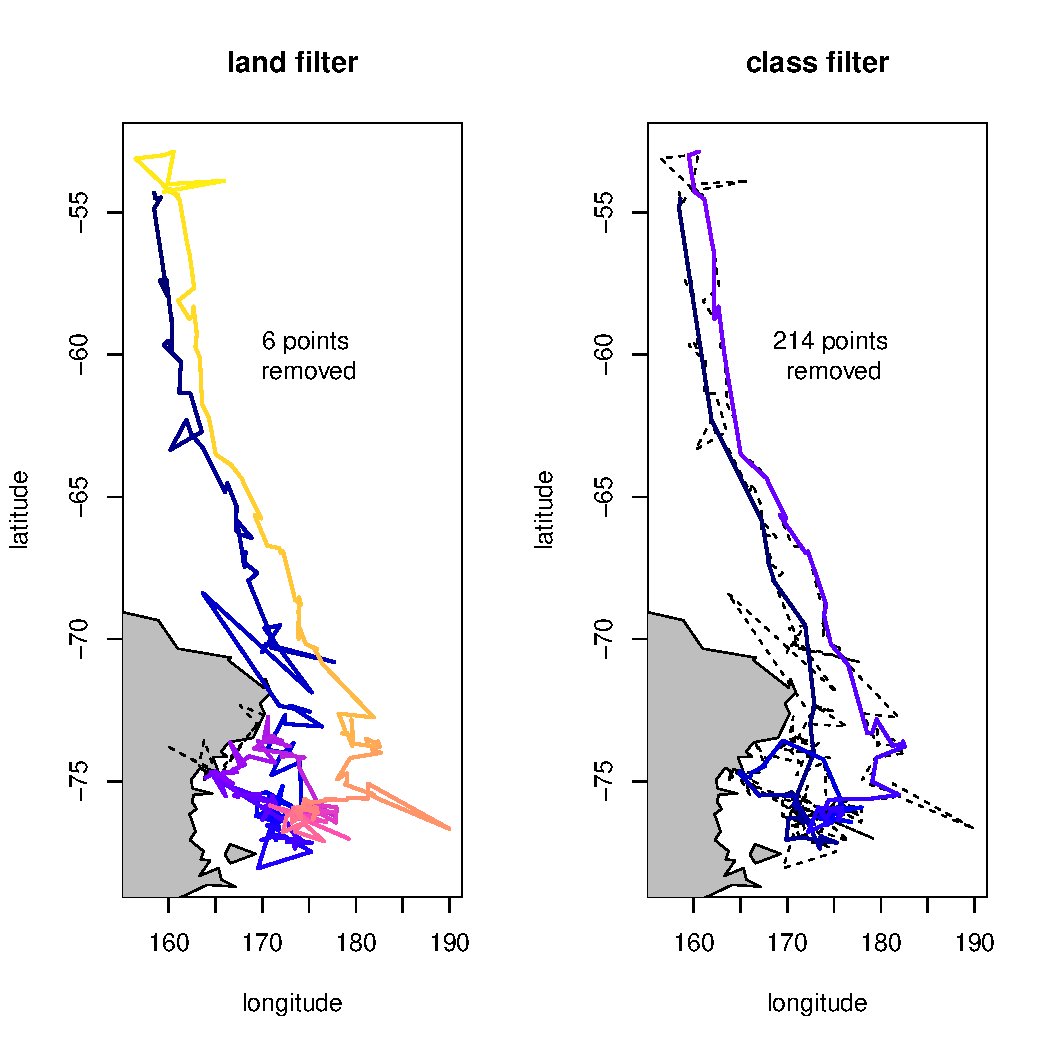
\includegraphics[width=\maxwidth]{figure/minimal-unnamed-chunk-3-1} 

}



\end{knitrout}
\end{center}
\caption{Land filter and Argos quality class filter (> B). In each
  panel the state of the track prior to filtering is shown
  as a dotted line. }
\label{fig:LandClassFilter}
\end{figure}

In the first panel the original track has been filtered for points on
the land area, and the second for points that have a location
quality class of ``B'' or lower. The land filter only applies to six
points in the track, but the class filter has removed 214, which is a
majority of the available 351 points.  The effects that these filters
have are independent of one another and it would not matter which were
performed before the other, although the result may be quite different
in combination that in the use of either one alone.

In terms of the land mask, the filter succeeds in removing points from
land but there is still a line segment that crosses a portion of the
Antarctic continent. A filter that applies to points is quite
different to one that applies to a continuous line segment. The class
filter provides a very cleaned-up track but at the expense of
discarding more than half of the available data.

The next example demonstrates a recursive speed filter applying the
method of \cite{MCF92} to the Argos track. This technique specifies a
running root-mean-square (RMS) summary of speed calculated by
determining the instantaneous speeds for each point to each of its two
previous and next locations. The RMS is defined as the square root of
the mean of the speeds squared. Any sequence of locations with an RMS
exceeding the maximum speed value have the peak RMS location discarded
and the RMS is recalculated. This continues until all locations have
an RMS less than the maximum speed. The threshold applied in this
example is 12 km/h.  Again the track is presented as
longitude/latitude coordinates with distance measurements calculated
relative to the WGS84 ellipsoid.

In the left panels of Figure~\ref{fig:SpeedFilter} are two plots of
the RMS values, for the second iteration after some positions are
removed and the sixth iteration when only a few nearby positions
remain above the threshold. The unfiltered RMS values are shown as a
grey line representing the original points, the current points that
have RMS values above the maximum are shown as crosses and the points
below the maximum are shown in faded black. The threshold speed is
shown as a horizontal line. As successive peaks of RMS values above
the maximum are removed the categorization for the remaining points
changes. This filter took ten iterations to remove all of the 73
offending locations, and the resulting track is shown in the right
panel.

\begin{figure}
  \begin{center}
\begin{knitrout}
\definecolor{shadecolor}{rgb}{0.969, 0.969, 0.969}\color{fgcolor}

{\centering 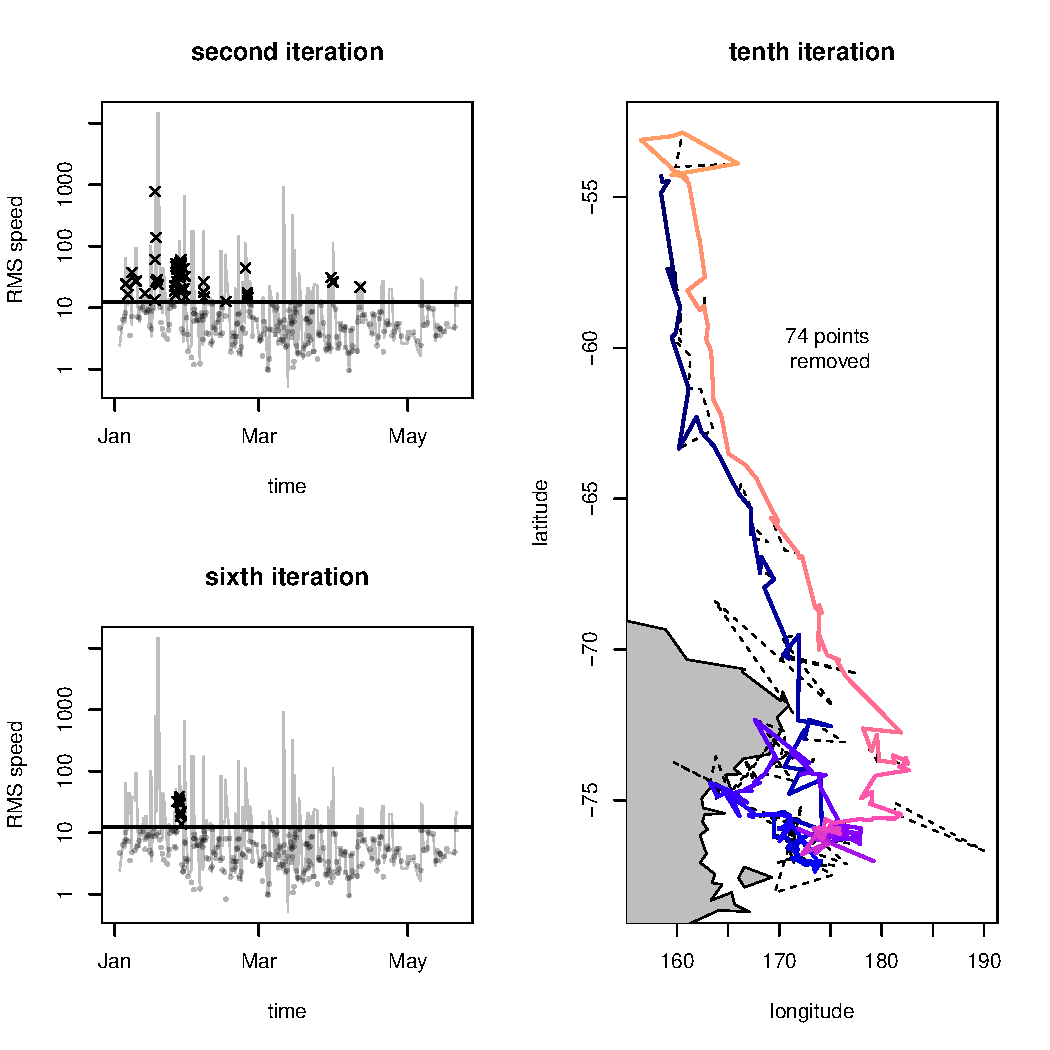
\includegraphics[width=\maxwidth]{figure/minimal-unnamed-chunk-4-1} 

}



\end{knitrout}
\end{center}
\caption{Recursive speed filter applied using the McConnell method. The left
  panels show the classifications provided for each point (RMS above
  the required maximum speed). The RMS speed axis is logarithmic.  }
\label{fig:SpeedFilter}
\end{figure}

This result seems reasonable, though there is no end to the complexity
and arbitrary nature of the decisions to be made. There are practical
uses for techniques like these however. Speed filtering can give a
reasonable result and there is a need to quantify the limits
here with comparative studies of various algorithms on known
data sets.

There are more sophisticated filtering algorithms that apply a suite
of tests. A published speed-distance-angle filter first removes a
minimum class (such as Z), filters for speed with the McConnell
algorithm and then recursively removes further offending points that
have a combination of acute angles and long implied distances
travelled \citep{freitas2008simple}. However, the accompanying
software is quite specific and unrelated to other packages. In Section
\ref{sec:tripdemo} a speed-distance-angle filter is created from
scratch using tools available in the \pkg{trip} package.

Related filters applying a combination of metrics have been published
by \cite{douglasfilter}, \cite{Taylor:BIRD} and \cite{AMB2}. The
algorithm published by Austin is available in the \proglang{R} package
\pkg{DiveMove} \citep{diveMove} and those by \cite{freitas2008simple}
and \cite{MCF92} in \pkg{argosfilter}. \cite{freitas2008simple} gives
an overview of the relative merits of various techniques, and the need
for hierarchical techniques to avoid discarding good quality
locations.

Another decision process is to choose between two possible locations
for each time step provided by the Argos Service in the DIAG format
\cite{Argos:MAN}. The Douglas Argos-Filter Algorithm applies this as
part of the filter \citep{douglasfilter}.

% <<>>=

% ## cols <- col.fun(length(ok))
% ## plot(coordinates(tr), type = "n")
% ## for (i in 1:10) {
% ##     ts <- ok[[i]] <= 12.5
% ##     ts[is.na(ts)] <- TRUE
% ##     lines(coordinates(tr)[ts,], col = cols[i], lwd = 2)
% ##     scan()
% ## }
% ## plot(fp[[1]]$rms, log = "y")
% ## ## plot up long/lat individually,
% ## plot.new()
% ## par(mfcol = c(2,1))

% ## plot(tr$gmt, crds[,1], xlab = "time", ylab = "longitude", type = "l")
% ## abline(v = tr$gmt[!sf], col = rgb(190, 190, 190, 190, max = 255))
% ## lines(tr$gmt, crds[,1])
% ## lines(tr$gmt[sf], crds[sf,1], col = "blue")
% ## plot(tr$gmt, crds[,2], xlab = "time", ylab = "latitude", type = "l")
% ## abline(v = tr$gmt[!sf], col = rgb(190, 190, 190, 190, max = 255))
% ## lines(tr$gmt, crds[,2])
% ## lines(tr$gmt[sf], crds[sf,2], col = "blue")

% ## ## windows()
% ## ##  p4 <-  "+proj=laea +lon_0=174.5 +lat_0=-65.5 +units=km"

% ## ## crds.p <- project(crds, p4)
% ## ## par(mfcol = c(2,1))
% ## ## plot(tr$gmt, crds.p[,1], xlab = "time", ylab = "x", type = "l")
% ## ## plot(tr$gmt, crds.p[,2], xlab = "time", ylab = "y", type = "l")

% @
\subsection{Non-destructive filtering}
\label{sec:penalty}

Non-destructive filters aim to update track points by some mechanism
without removing corresponding data records. There are many examples
such as algorithms to modify light level geo-locations for latitude
with SST \citep{BM02} and interpolative techniques to smooth tracks
\citep{TSF06}. Many destructive filters can be recast in a
non-destructive form using a penalty smoothing approach in the style
of \cite{roughpenalty}. For example, rather than filter the track to
exclude locations that would imply an unrealistic speed of travel, the
track can be smoothed using a speed of travel penalty.  The smoothed
locations are determined by minimizing the functional
\begin{displaymath}
  J_{\lambda}(\hat{x}) = \sum_{i=1}^{n} d(x_{i},\hat{x_{i}})^{2} +
  \lambda \sum_{i=1}^{n-1}
  v(\hat{x}_{i}, t_{i}, \hat{x}_{i+1}, t_{i+1})^{2}
\end{displaymath}
where $\{x_{1}, \ldots, x_{n}\}$ represent the raw (unsmoothed)
locations, $\{\hat{x}_{1}, \ldots, \hat{x}_{n}\}$ their smoothed
counterparts, $d(x,y)$ represents the distance from $x$ to $y$, and
$v(x,t_{x},y,t_{y})$ the speed required to travel from $x$ at time
$t_{x}$ to $y$ at time $t_{y}$, and $\lambda$ is the smoothing
parameter. The first term is a measure of goodness of fit of the
smoothed locations $\hat{x}_{i}$ to the raw locations $x_{i}$, while
the second is a speed penalty.  Minimizing $J_{\lambda}$ trades off
goodness of fit against speed of travel.  When $\lambda=0$ the
smoothed track reproduces the raw track exactly.  Increasing $\lambda$
favours tracks requiring less extreme speeds, at the expense of
reproducing the $x_{i}$.

As for the more traditional application described by
\cite{roughpenalty} this process can be interpreted in a Bayesian
context. Adopting a penalty based on squared speeds is equivalent
to adopting a Gaussian prior on speeds, adopting a penalty based
on the absolute values of speed is equivalent to an exponential
prior on speed.

An application of this non-destructive filter was applied to the
example Argos data set discussed earlier. Figure~\ref{fig:PenSStrack}
shows the filtered result on a map and Figure~\ref{fig:PenSSLonLat}
shows the same result with longitude and latitude plotted against
time. The result seems reasonable with a plausibility comparable to
that of the recursive speed filter with the advantage of not having
removed any data from the trip.


% \subsection{Non-destructive filtering}
% \label{sec:penalty}
% Non-destructive filters aim to update track points by some mechanism
% without removing the data record. There are many examples such as
% algorithms to modify geolocations for latitude with SST \citep{BM02}
% and interpolative techniques to smooth tracks
% \citep{TSF06}. Techniques used for destructive filtering can be recast
% by penalizing the fit of the smooth track fit to the original
% locations by a calculated metric. The following example smooths using
% a roughness penalty approach \cite{roughpenalty}. The smoothed
% locations $\hat{x}_i$ are determined by minimizing the functional
% \begin{displaymath}
%   \operatorname{V}\left (\hat{x}_{i}, t_{i}, \hat{x}_{i+1}, t_{i+1}
%   \right)^Z \beta_{\lambda}
% \end{displaymath}

% [spoon to finish]

% Here $\{x_{1}, \ldots, x_{n}\}$ represent the raw (unsmoothed)
% locations, and $\{\hat{x}_{1}, \ldots, \hat{x}_{n}\}$ their smoothed
% counterparts; represents the distance from x to y, and V the velocity
% required to travle from x at time tx to y at time ty. Minimizing J
% balances the accuracy with which the smoothed locations xhat reproduce
% the raw locations $x_i$, against the velocity required to traverse track
% segments. Decreasing lambda favours reproducing the raw locations,
% increasing lambda favours tracks requiring less extreme velocities, at
% the expense of reproducing the $x_i$.

% As for the more traditional application described by
% \cite{roughpenalty} this process can be interpreted in a Bayesian
% context. Adopting a penalty based on squared velocities is equivalent
% to adopting a Gaussian prior on velocities, adopting a penalty based
% on the absolute values of velocity is equivalent to an exponential
% prior on velocity.

% Figure~\ref{fig:PenSStrack} shows the filtered result for the example
% Argos data set. Figure~\ref{fig:PenSSLonLat} shows the same result
% with longitude and latitude plotted against time.


% The following example applies
% nonparametric smoothing using a roughness penalty approach
% \cite{roughpenalty}. Using the sum of squared velocities is equivalent
% to placing a guassian penalty on the velocities, and using the
% absolute values would be similar to an exponential penalty. The
% non-linear minimization techniques used are highly sensitive irregular
% time values and so some sort of resampling to produce tracks with
% regular time intervals is required.


\begin{figure}
  \begin{center}
\begin{knitrout}
\definecolor{shadecolor}{rgb}{0.969, 0.969, 0.969}\color{fgcolor}

{\centering 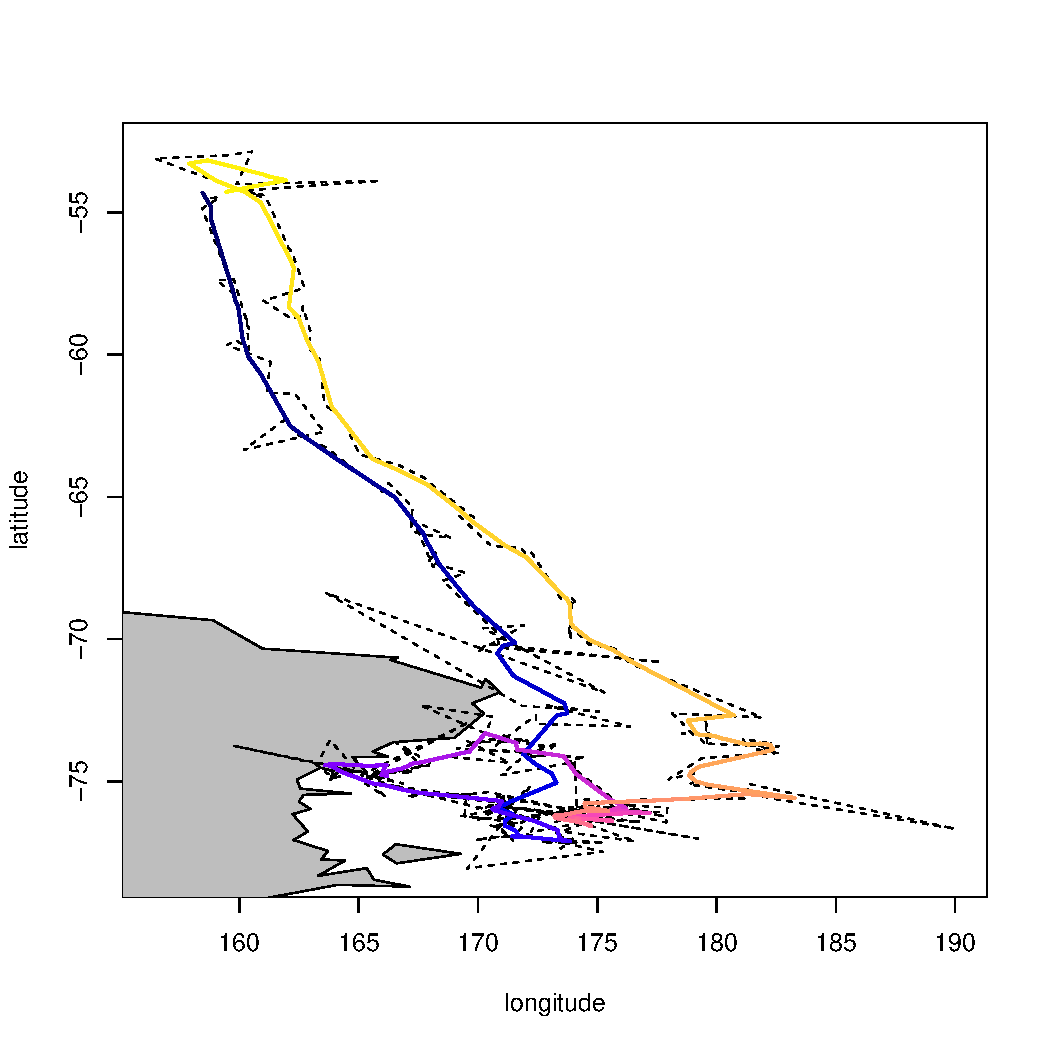
\includegraphics[width=\maxwidth]{figure/minimal-unnamed-chunk-5-1} 

}



\end{knitrout}
\end{center}
\caption{Argos track filtered by penalizing by sum of squares
  speed. The original data was used without resampling}
\label{fig:PenSStrack}
\end{figure}


\begin{figure}
  \begin{center}
\begin{knitrout}
\definecolor{shadecolor}{rgb}{0.969, 0.969, 0.969}\color{fgcolor}

{\centering 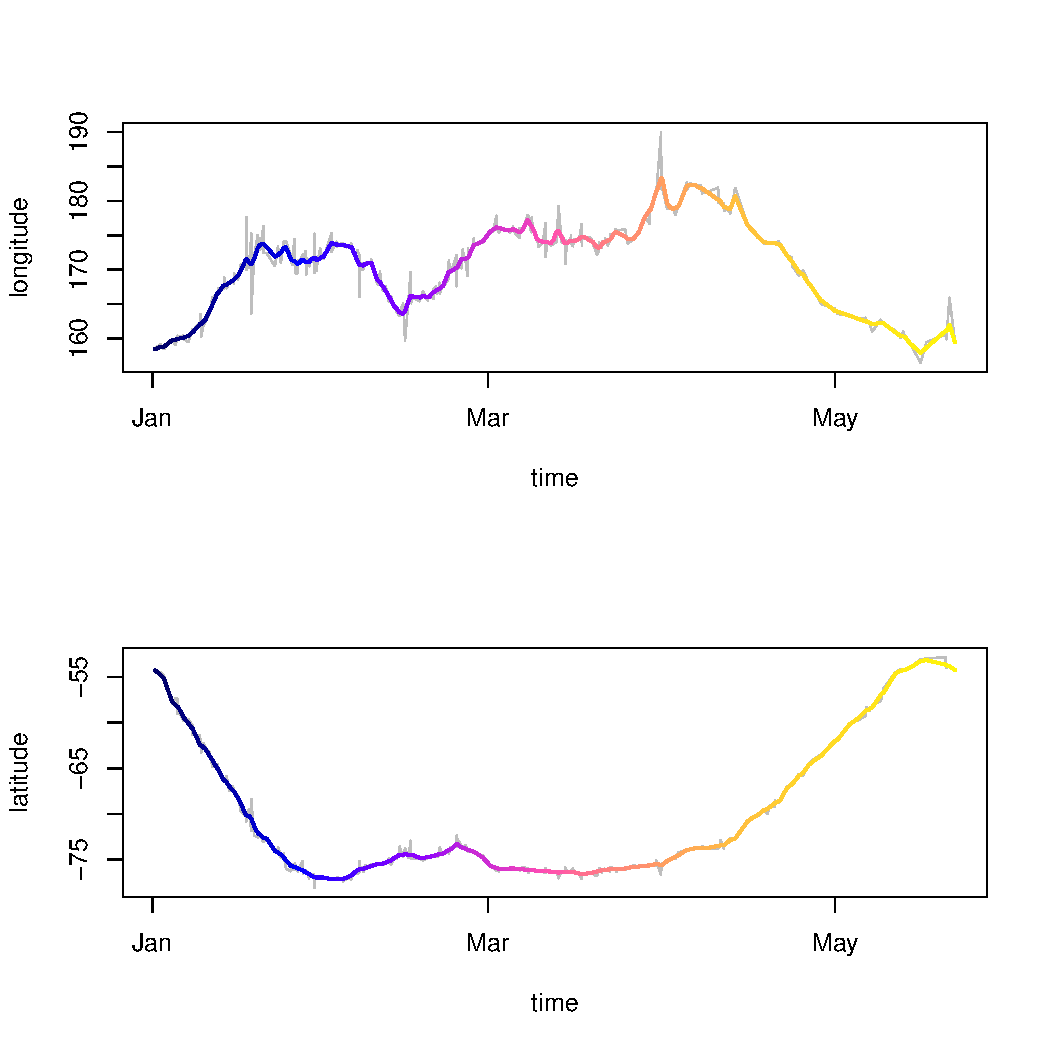
\includegraphics[width=\maxwidth]{figure/minimal-unnamed-chunk-6-1} 

}



\end{knitrout}
\end{center}
\caption{Penalized sum of squares speed---track longitude and
  latitude. }
\label{fig:PenSSLonLat}
\end{figure}


%Kalman filters, state-space etc. - usually non-destructive?
\subsection{Spatial smoothing---surfaces from track data}
\label{sec:surfaces}
There are a number of ways of creating bivariate (surface) estimates
from track data, the most common involve a surface defined by a grid
of cells or connected points. (Regular grids are historically easy to
store and to compute, and so are applied most commonly---irregular grids
and meshes are not considered here). The most direct methods are
variously called ``rasterization'', ``gridding'' or
``pixellation''---these effectively generate a bivariate histogram
from the input point or line data. Kernel methods apply a bivariate
distribution (such as a Gaussian) to the input points or lines. Point
methods are not discussed here, but can be achieved in a similar way to
the line-based examples shown in Section~\ref{sec:tripdemo}.

The following is a very simplified folk history of tracking
techniques, but does help explain some of the existing practices that
differentiate terrestrial and marine applications. There is an
apparent difference between terrestrial and marine applications in the
way that surface creation, or gridding methods are applied. Terrestrial
applications tend to ignore time or adapt data to avoid temporal
auto-correlation. VHF techniques were the original primary tool for
wildlife tracking, and the metric of interest was pure residency---the
minimal region in which the animal is present (home range) and the
animal's core region. In this context actual ``tracks'' are not the
main interest. Marine applications have traditionally been explicitly
interested in tracks and the temporal relationships, perhaps because
of the real and perceived differences in the dynamics of marine
environments. Modern techniques are seeing a far greater cross-over in
these originally different fields and the differences are now out-weighed
by the common goal of reliable location estimation.

%% https://stat.ethz.ch/pipermail/r-sig-geo/2010-September/009283.html

Cell binning and kernel density estimation (KDE) can
unproblematically convert a linear geometric track representation into
a 2D histogram-like smoothing of residency, time spent map, or other
utilization distribution but both must grapple with serious problems
of interpretation. Points and lines simply do not represent the
movement of an animal completely. Both methods must deal with
issues of independence, point or line interpretations and complex
boundaries and environmental relationships. If these issues can be
dealt with or ignored, both cell gridding or KDE can be used as a
convenient smoother for track data.



% Point
% interpretation, line segment interpretation, KDE scale independence,
% time-spent max-depth drift-rate - further overlays with
% enviro. Multiband grids, multivar models.  - use Hindell's MDBs to
% find a good example.  - weighted variance for location quality,
% weighted amplitude for time difference



The following combinations of methods are applied in various ways in many
existing publications. The grid surface is generated by operating on
points or on line segments. Line segments provide a continuity
through space and so they provide a natural way to connect regions
visited by the animal. Lines present a harder problem to convert to a
grid than points and so this is often approximated by providing
interpolated points in place of line segments, assuming constant
travel speed.

%% contribution to the surface
The influence of the points or lines on the surface is calculated by
binning into the overlapping grid cells directly, or by calculating
the contribution to neighbour cells via a ``kernel''. In the case of
binning, the coverage provided by overlay with cells is not great,
leading to a requirement for larger bin sizes, compromises balanced
against positional accuracy and the need to match with covariate data
\cite{BHMS02}. The limitations here are the same as those for
histograms in general---the discontinuous histogram presents
analytical difficulties as it quite senstive to the chosen origin, bin
size and orientation
\citep{simonoff1996smoothing,silverman1998density}. Kernel density has
the advantages that the result is smooth without the blocky,
discontinuous nature of a bivariate histogram. Regular or irregular
``wireframe'' representations give a smoother result and have
continuous analytical and visualization counterparts via
interpolation, but these data structures are more complicated to
calculate and are much less widely supported.

%% weighted by time, accuracy or something?
Finally, when the cell value is determined there are various ways in
which the contribution of a point or line can be calculated. The point
or line can simply be summed into the cell---a point is counted
as present in the cell whereas the proportional length of an overlapping line
segment is added to the bin. Each bin contribution can be multiplied
by a factor, such as a point value or the time interval available to
a line segment. This is one of the natural cases for using line
segments from track data rather than points, as when the duration of
time is of interest the input points cannot represent the duration of
time. Many studies approximate this by creating a regular time series
by interpolation.

When kernel density methods are applied, a weighting factor can be given
for either dimension of the kernel, or more generally a
two-dimensional correlated weighting is used
\citep{simonoff1996smoothing}.

The following examples show the gridding of a very simple track by
some different methods.


\subsubsection{Exact gridding}
\label{sec:exactgridding}
Gridding (pixellation or rasterization) methods generate a grid of
cells that extend completely over the region of input track data.


A very simple track is shown in Figure~\ref{fig:coarseGrid} with an
underlying grid. Each line segment has a value assigned to it, the
time duration between each track point. These values are [2, 3, 1, 7,
1, 1] and the first and last line segments are quite long, so their
contribution to the cells is small relative to the middle
segments. This is reflected in the grid, which represents the implied
``time spent'' in each cell. In order to determine the contribution of
each line segment's value to a cell, the segment is split on the
boundaries of the cells that it crosses and the value shared
proportionally based on the length of the resulting
segment-portion. This computation is not simple---to describe it in
GIS terms this is an overlay of the line and the cells (``topology
overlay'') with a rule to transfer values from the lines to the cell,
in this case a proportional sum. GIS can be used to perform these
calculations, but as discussed in Section~\ref{sec:software} working
with time in GIS is not well supported and this must be done as an
attribute on line objects, rather than on inherently continuous lines
that vary through time or other dimensions as well as space.


\begin{figure}
\begin{center}
\begin{knitrout}
\definecolor{shadecolor}{rgb}{0.969, 0.969, 0.969}\color{fgcolor}

{\centering 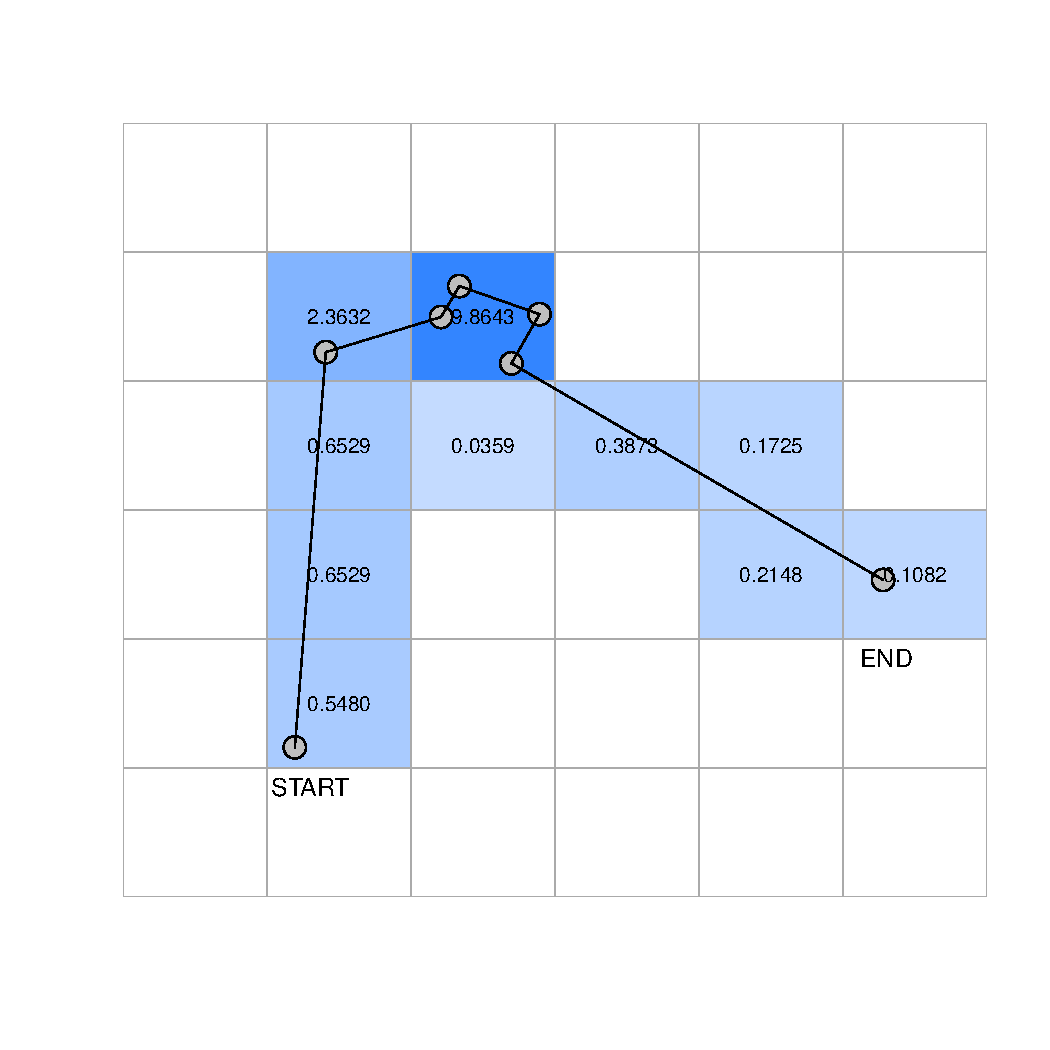
\includegraphics[width=\maxwidth]{figure/minimal-unnamed-chunk-7-1} 

}



\end{knitrout}
\end{center}
 \caption{Track lines binned into a coarse grid, using a line segment value
   to sum into each cell. Cells are coloured from light to dark blue
   for increasing values. The sum of values resulting from each
   smaller line segment is shown for each cell. }
 \label{fig:coarseGrid}
\end{figure}

The dependence of the gridding method on bin size is easy to
see. Figure~\ref{fig:fineGrid} shows the same gridding process applied
to a finer grid, with the same origin. The grid again completely
summarizes the contribution of the track, but the actual regions
influenced by the grid are quite different---the small grid cells
snugly trace the track and cover a much smaller overall area than in
the case of the coarse grid. The total time duration represented by
the coarse and fine grid is exactly the same, but the results are
quite different.

This dependence on scale has been used explicitly to provide a compromise
between positional accuracy and spatial coverage with the need to
match with environmental data by \cite{BHMS02} and
\cite{burns2004winter}. \cite{BHMS02} also explicitly used grid size
to help acccount for spatial uncertainty.  As discussed previously the
assumptions made by these analyses become substantial, involving
issues such as uniform location accuracy, uniform grid scale and
constant straight line travel.

\begin{figure}
\begin{center}
\begin{knitrout}
\definecolor{shadecolor}{rgb}{0.969, 0.969, 0.969}\color{fgcolor}

{\centering 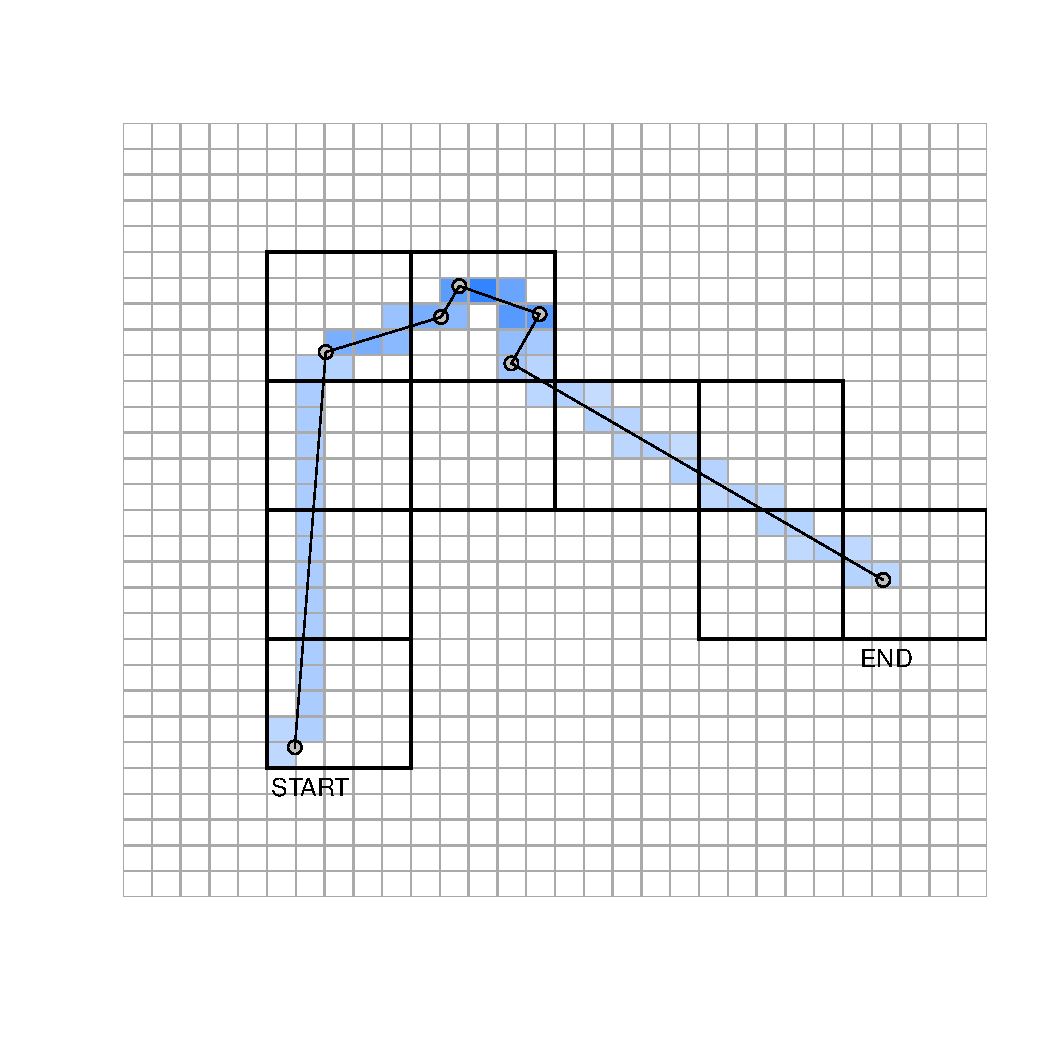
\includegraphics[width=\maxwidth]{figure/minimal-unnamed-chunk-8-1} 

}



\end{knitrout}
\end{center}
 \caption{Track lines binned into a fine grid. The track and grid
   origin is the same as in Figure~\ref{fig:coarseGrid}. The coarser
   grid outline is shown for occupied cells as thick black lines. }
 \label{fig:fineGrid}
\end{figure}

\subsubsection{Kernel density methods}

Kernel density methods are applied to overcome the dependence of the
probability density function on the origin and bin size, as it is the
properties of the kernel that dictate the contribution to each cell.
(In theory every input point or line contributes to every cell to some
degree). The result is thus less related to the data structure
choices, given a sufficiently fine
resolution. Figure~\ref{fig:coarseGrid3D} shows the same coarse simple
grid with an equivalent KDE grid in a perspective plot. The KDE result
is still blocky, but the overall value of the surface is continuous,
and not restricted to regions near the line. By increasing the
resolution, the continuous nature of the KDE approach becomes more
apparent---this is shown in Figure~\ref{fig:fineGrid3D}, again
equivalent to the vertical view of Figure~\ref{fig:fineGrid}.

Kernel methods are more commonly used in terrestrial home-range
applications than marine applications, perhaps as the measure of
interest is a spatial region, rather than the actual trajectory of the
track. Explicit line-to-cell methods have been used in marine
applications because of the focus on time spent based utilization
distributions. There is a convergence of aims here that is still
developing, and is seeing resolution in modern statistical methods.


Kernel density methods are commonly applied to track data because of
these advantages, but perhaps due to implementation difficulties with using
line segments published applications use an equal-time interpolation
between track points \citep{Taylor:BIRD}.

The \pkg{trip} package provides tools to produce simple and KDE grids
with line or point interpretations. The distinction here is one
between discrete and continuous representations which can be
represented in the data itself, or in the visualization technique or
analysis used. The lack of clarity for these distictions in spatial
software is one of the problems faced in tracking research.

Other approaches have tended to use the locations more directly, by
categorizing them as belonging to ``focal foraging areas''
\citep{simmons2007linking} or with ``first passage time'' analysis
\citep{Pinaud2007}.


% Full code examples are provided in
% Appendix B? Also illustrated in Appendix B? are histogram-like cell
% ``tower'' plots versus mesh-like ``wireframe'' plots.



% STAT tool:
% http://www.int-res.com/articles/feature/m301p001.pdf

% \cite{Coyne2005} paper with shared goals of helping researchers do
% their work.

% On the need for exploratory analysis, and purpose-built tools for
% tracking data:
% \cite{dray2010exploratory,calenge2009concept}


% line segments

% bivariate histogram - coarse / fine
% bivariate kde - coarse / fine

% - discuss issues of scale and coverage
% - discuss GIS-like overlay to cut lines into partial segments

%   points only / points interpolated

% bivariate hist - fine
% bivariate kde - fine

% - discuss that interpolation can be used to extend points to approx lines

% Mention different representations, wireframe/histogram of cell/continuous but put in
% appendix.


\begin{figure}
  \begin{center}

    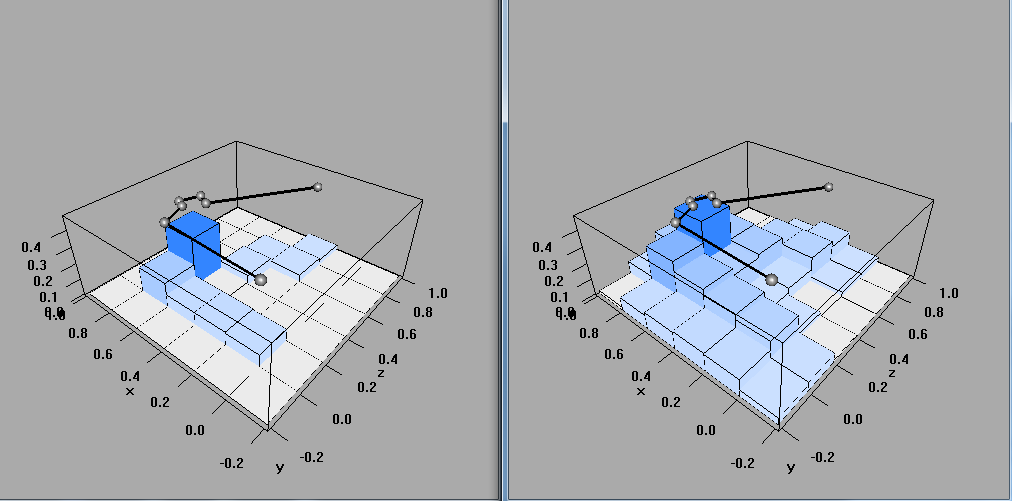
\includegraphics{figures/3Dplots-coarseGRIDvsKDE.png}

    \end{center}
 \caption{Side by side plots of line gridding and KDE gridding to a
   coarse grid. The
   input line is shown at an arbitrary height above the cells.  }
 \label{fig:coarseGrid3D}
  \end{figure}



\begin{figure}
  \begin{center}

    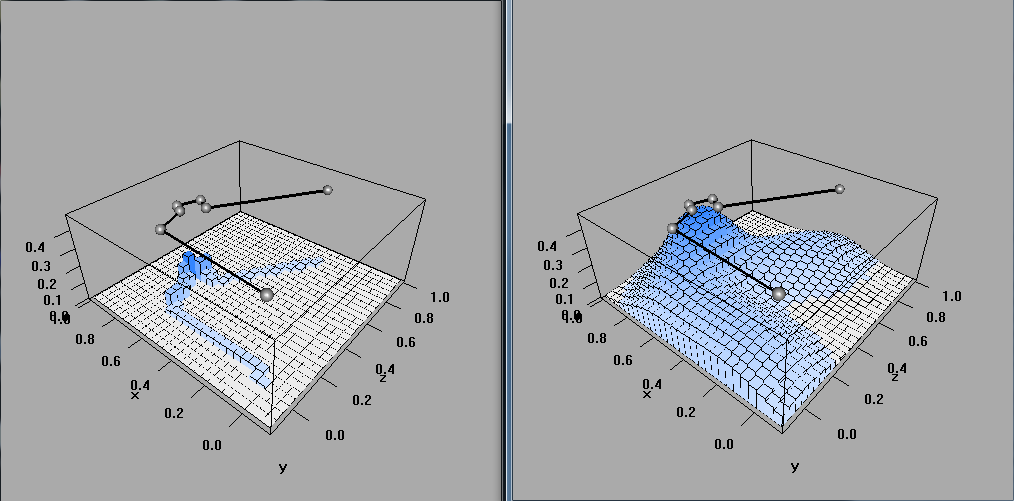
\includegraphics{figures/3Dplots-fineGRIDvsKDE.png}

    \end{center}
 \caption{Side by side plots of line gridding and KDE gridding to a
   fine grid. The
   input line is shown at an arbitrary height above the cells.  }
 \label{fig:fineGrid3D}
  \end{figure}



\subsubsection{Attribution of point or line values}
Time duration between measured locations is a common value of
interest, but many others may be used such as drift dives
(e.g. \cite{thums2008tracking}), maximum depth, temperatures encountered,
etc. The \pkg{trip} package provides tools to apply arbitrary values to
gridding methods by providing conversions between point and line based
interpretations and the ability to store multiple attribute values for
points and lines.


\subsection{Partitioning tracks and grids into time periods}

Gridding methods are easily applied to entire tracks by
binning into a single grid. In order to partition track data into time
periods the lines (or other approximation to continuous path) must be
cut into time durations. This requires that the path be cut at a point
intermediate to the input points as these will rarely coincide with
the period boundaries.


Once the trips are cut into exact time boundaries summaries derived
from them represent some form of 3D grid in order to represent each
time period separately. The track line must be cut exactly at the
time boundaries, assuming constant travel speed and the contribution
of each part summed separately into two grids. The \pkg{trip} package
provides tools to partition sets of tracks in this way and generate
collections of spatial grids. Using the simple methods above the trip
data can be partioned in time to give temporal-based utilization
distributions \citep{keating2009modeling}.

A more general method of representing arbitrary time periods from
modelled tracks is discussed in Chapter~\ref{chapter5}.


% Cutting tracks into temporal partitions is important for many studies,
% and while categorizing point locations into time periods is very
% simple, the line interpretion often requires that the lines be cut at
% a point intermediate to point locations. Effectively, new coordinate
% must be inserted at a point based on linear interpolation. The
% \pkg{trip} package contains functions for splitting trips at exact
% temporal boundaries, which can then be processed into grids. Multiple
% time periods for a study are then simply manipulated as a
% multi-attribute grid or a 3d array using the basic spatial tools in
% \proglang{R}.



% \begin{figure}
%   \begin{center}
%  <<print=FALSE,echo=FALSE,fig=TRUE>>=
% g <- GridTopology(c(-0.1, -0.1), c(0.2, 0.2)/3, c(16, 16))
% pgs <- as.SpatialPolygons.GridTopology(g)
% tripGridEG(exact = TRUE, main = "B", cex = 0.6)
% @
% \end{center}
% \caption{  }
% \label{fig:}
% \end{figure}



% @
% \end{center}
% \caption{  }
% \label{fig:}
% \end{figure}


% \begin{figure}
%   \begin{center}
% <<print=FALSE,echo=FALSE,fig=TRUE>>=

% @
% \end{center}
% \caption{  }
% \label{fig:}
% \end{figure}




% We present various simple ways of summarizing behaviour with track
% data.  To illustrate the ideas and techniques applied for solving
% various problems, which we see solved in an integrated fashion using a
% Bayesian approach. The software used in these examples is available from [MDS etc.]
% in R packages.  [Code for examples in Appendix?  Give descriptions of data used, QC and
% metadata - classes, length etc of data]
% Ad hoc approaches to track location involve some form of filtering
% for quality, and then using those points in time to summarize
% behaviour.  Here we describe some of the simple methods in use, relate
% their rationale to other methods available, and document the
% conceptual steps we took based on their limitations.

% \subsection{Prosaic issues}
% Is this really necessary?

% % Creating time spent maps of
% % foraging behaviour for marine animals is a relatively simple exercise,
% % but there are a number of problems that are worth capturing in defined
% % programming constructs.  A common case involves a tabular file (text
% % or Excel) containing a set of records of dates, times, longitudes,
% % latitudes, animal id, trip id, and various other data. In the minimum
% % case I use the trip class from package timeTrack to summarize these
% % data.  Rather than describe how R is used to do it, I will describe
% % the steps taken conceptually. First the data require a sensible
% % organization into individual trips. This is fairly obvious, with the
% % basic case being an animal that was ``captured'' and tagged, then
% % ``released'' whence it took off on a foraging ``trip''. On
% % ``recapture'', or otherwise remotely accessed data from the tag the
% % spatial features of the trip are of interest and can be determined
% % from tag data. Within individual trip identities the records must be
% % in temporal order in terms of the dates and times, with the further
% % proviso that there exist no duplicate times. Assuming the data are
% % correct, a simple (re-)ordering of the records suffices but in the
% % case of duplicates a decision must be made. By default I adjust any
% % duplicate date time location record (note that I assume that fully
% % duplicate records contain zero information, and so they are discarded
% % as a artefact) by adding a second to the subsequent date time.  (This
% % is not robust to cases where there is a series of duplicates, or
% % sufficiently near records, but this seems to be so rare as to not
% % worry about).


% \subsection{Destructive filtering - speed, angle, distance, class, masks}

% % \\ The next step is to remove obviously bad location
% % estimates, of which there are usually some. One thing that can be done
% % is to select the individually and discard, or select records below
% % some specified location ``class'', or to remove any locations on land,
% % or etc. A common automatic step is to ``filter'' the data based on the
% % implied speed between fixes.

% As discussed above, the process of removing locations from a track can
% improve the result but there is no absolute level at which to
% determine the correctness of a particular location. The filtering will
% always be susceptible to a cut-off point where a point should be
% discarded or retained.

% Destructive filters aim to improve the quality of a set of points by
% removing locations that fail a simple movement test. The most commonly
% used techniques are based on speed, angle, distance and masks. Speed,
% angle and distance filters define threshold values at which a point is
% discarded and each require a method of calculating an appropriate
% value for each point. These methods are described separately, although
% in practice they are used in combination. Combining these methods
% presents a new class of definition problems over the ones faced by
% each method itself.

% For a speed filter, speed can be calculated in a number of ways. The
% most salient values are the speed to the point from the previous
% point, and the speed from the point to the next point. A decision must
% be made regarding the first and last points, which have only one
% instantaneous speed available to them, and further each point removed
% then changes the remaining metrics by which the other points are
% assessed. To deal with this recursive problem McConnell introduced a
% speed filter that calculates a root-mean-square (RMS) of instantaneous
% speed for each location based on the two previous and and two next
% points. Locations above a given threshold are removed, the RMS is
% recalculated and the process repeats until all RMS values are below
% the threshold. This method was published in [1992], and made available
% as an algorithm implemented in IDL by David Watts [pers. comm. and
% AWRU website], and in function speedfilter() in package
% 'trip'. [Taylor] presented a variation on the methods that calculated
% speeds from the point to the previous and next, and from the point to
% second previous and second next points, rather than using the
% sequential steps.  Sebastian Luque also published a version of the
% McConnell filter (non-recursive) in package 'diveMove'.

% More detailed versions including speed, distance and angle available
% in R package 'sdafilter'.

% \begin{figure}[!ht]
%   \begin{center}
%     \includegraphics[width=120mm]{roughfigures/filteredC993Argos.png}
%   \end{center}
%   \caption{
%     {\bf Raw Argos estimates filtered by speed}
%   }
%   \label{FigrefFilteredArgos}
% \end{figure}


% \subsubsection{Filtering}
% Locations may be chosen based
% on their Argos quality, by a running mean of speed below some minimum,
% or by a combination using the Argos diagnostic information. Arguably, any
% data set of locations and times may be imagined as having auxiliary "quality"
% information for each record.  This might be service-supplied (e.g. Argos classes), or
% derived from the data themselves (filters for speed, angles etc.).  The use
% of these metadata could be as destructive filters, or somehow as weights for
% determining more reliable records---or to simply tag records that need some
% user-assessment or correction.  As distinct
% to actual destructive filtering, correction algorithms exist to hone a
% location component (usually latitude) using environmental data -{} SST
% is the classic example \cite{BM02}(Snake, KJM, Rick,
% Beck, ...). Our fundamental objection to this kind of correction is that one
% source of information is discarded in favour of another, where both ought to be
% used.

% General geolocation based on other data, examples.



% \subsection{Non-destructive filtering}
% Discarding data is avoided by these methods, but the fundamental
% problem is a lack of a realistic model of the process. The techniques
% tend to take the ``join the dots'' model and modify it using geometric
% techniques (ref Patterson for related critique).

% Spline smoothing methods. Bezier curves (Tremblay). Penalized sum of squares.

% \begin{figure}[!ht]
%   \begin{center}
%    \includegraphics[width=120mm]{roughfigures/smoothC993Argos.png}
%   \end{center}
%   \caption{
%     {\bf Smoothed Argos estimates}
%   }
%   \label{FigrefSmoothedArgos}
% \end{figure}


% \subsection{Spatial smoothing for utilization distributions}
% Cell methods effectivly assume linear motion between points and solve
% for the proportion of each line segment falling in each
% cell. This assumes that each line segment represents a continuous path
% at regular time. Direct cell methods like this suffer the problem of
% what cell size is appropriate. Other methods like kernel density
% estimators are not constrained by this choice of cell size, but
% introduce further problems about what points to include in the kernel
% (the track nodes, or points along a line segment) and how to weight
% for the difference in time between points. (An approach applied to
% cell and kde methods is presented below in \ref{sec:?}).

% Given the problems of location uncertainty, the need to match cell
% grids to environmental data, and the problems in spatial coverage of
% environmental grids the work of Bradshaw aimed to find the right
% compromise cell size.


% Geometric summaries such as binning time spent into cells can give
% useful guides for further analysis, but they also can present more
% difficult problems. What do we bin? Track points can be binned
% directly by a simple count which assumes that each location has an
% equal ``weight''.

% Approximation techniques used in package 'trip'.

% Problems of spatial and temporal scale, often chosen to match environmental data.

% \begin{figure}[!ht]
%   \begin{center}
%     \includegraphics[width=120mm]{roughfigures/gridTimeC993Argos.png}
%   \end{center}
%   \caption{
%     {\bf Gridded Argos estimates}
%   }
%   \label{FigrefGriddedArgos}
% \end{figure}

% The difference between cell based time spent and kernel density
% methods. Kernel density is fundamentally inappropriate [this claim
% needs justification] for the problem, but is often used as it provides
% a simply-implemented smoothing technique.

% The following focuses on two commonly used aspects of smoothing
% discrete points for time spent, or ``utilization distributions'' to
% highlight salient issues. It is not a comprehensive summary of the
% variety of methods availalble. The immediate question that comes up
% when considering a gridding approach is that of the appropriate
% scale. If we choose a grid cell size that is too small, we diffuse the
% contribution of any particular location over too many elements and if
% the cell is too large the contribution from many locations are lumped
% together. Either way we will swamp the signal we are trying to
% discern.

% Given the problems with location accuracy, the cell size choice was
% used to find a compromise by matching the optimal cell size to a)
% capture the problems with location precision (a larger cell size is
% forgiving of point accuracy) and b) find a meaningful scale at which
% effort is being expended by the animal (the smallest cell size at
% which the animal is interacting with the environment). There are many
% problems with this approach: why should scale not be independent of
% location accuracy? how to compare different grid choices for different
% animals, species, regions, coordinate systems?

% * There is no theoretical reason why regular grids are used, or even
% why structured grids are used - these are surely just the result of
% convenience and the availability of tools.

% \subsubsection{Approximation to cell gridding}
%  The final step requires some more
% decisions, but it's worth noting that using R's features we have
% easily achieved the above steps by working on the full data table
% containing every animal's trip. The next step can be computationally
% demanding in terms of memory, so it makes sense to first split this
% large table for each trip, summarize for each separately and then
% merge these back together. The first decision is to choose some
% minimum time step to which we will interpolate points to measure time
% spent (this is easy to do algorithmically, rather than solve for
% durations between arbitrary lines). The shorter the time step the
% longer interpolation will take, but the more accurate will be the
% final balance of time spent. In practice 1 hour will work, but to be
% very neat we might choose 1 minute. Next we require a spatial grid to
% summarize time spent.  We choose a grid spacing (in kilometres - grids
% are created in lat/lon but are approximately true at the centre
% latitude, see below) and a grid extent if desired, but this can be
% determined from the points themselves. We then interpolate each set of
% trip locations so that we have (approximately) 1 position for each
% minimum time step, and then count the number of locations falling
% within each grid cell. Then we merely multiply these bin counts by the
% minimum time step, which is the simplifying step we mentioned above.
% These grids are simply matrices that we can then add together to get
% the full picture of time spent.

% \subsubsection{Partitioning tracks and time spent grids}
% The process of splitting the data can be generalized to many levels,
% we can split the data into sexes, or years, or seasons and create
% separate grids for each of these groups. If we require greater spatial
% rigour we can choose an appropriate projection, transform all the raw
% coordinate data to this and create our interpolation and grids based
% on this.


% \subsubsection{Kernel density methods} (KDE was introduced to address
% short-{}falls of home range?{})Home range analysis has a long history in
% animal tracking studies, and convex hull methods have been used to
% confine the area accessed.  The meaning and utility of home range is
% much debated, and it might be the case that the concept is more
% applicable to the terrestrial rather than marine environment. However,
% many marine cases are published where the same principles and techniques
% are applied[turtle stuff 2006?]. Obvious problems since animals actually
% follow a track, this is partly addressed by KDE since the density of
% locations measured will surely represent the concentration of effort.
% This is fine if the points are measured at equal intervals of time, but
% given that the quality of all locations is not equal this cannot be the
% case.  Points may be interpolated between those given to give equal time
% periods, but again there is a problem of uncertainty -{} calculating the
% increased range of possible movement becomes unweildy and arbitrary.
% Fancier means of interpolating using curvilinear techniques [Tremblay
% and co.] \texttt{may} provide a more natural or feasible shape of track,
% but the ability to determine reliability is not enhanced by such
% techniques. The uneven sectioning of time periods between points creates
% a new problem of assigning simple behavioural summaries such as time
% spent.  A covariate may be introduced with time differences between
% points, but the problem becomes one of where to centre that
% contribution. Mid-{}points are one possibility, or to interpolate using
% the speed of the animal between points with a moving window, . . . Many
% simple and sophisticated combinations of convex, triangulation, kernel,
% and other methods blah blah blah [Here I can show the stuff I did with (
% sm) package at Macq.]

% \subsubsection{Cell gridding}
% A well-{}intentioned solution to the lack of time as a covariate within kernel methods
% prompted the gridding technique.  The idea is to create a set of
% spatial cells in which to determine exact lengths of time by treating
% the line segments as the entity containing the information.  The line
% segments are assigned the time difference between their end points,
% then the lines are split by the grid cell boundaries.  This is an
% easily achievable operation using simple GIS techniques (ref?{}?{}), or
% by interpolating to an equal time spacing and simply determining point
% per cell counts.  The next step is usually to account for transit time
% that overweights the time spent close to the colony location. What is
% appropriate here will depend upon the animals and the desired analysis, but
% in general is probably best handled by carefully defining the start and
% end times of "trips" so that excess "home time" is not added to the picture.
% Perhaps some judicious exclusion of early and late trip times is the easiest
% way.  [What about with prob. methods - can you just look for massively
% transited areas automatically?]








% \section{Existing approaches - broad literature review with examples}
% Our purpose here is to present some of the more common techniques used
% to prepare and analyse data---partly to illustrate their use and rationale,
% but also to provide some tools for their implementation.

% %% This examples section should work through the problems faced in
% %% real conditions, and then through the ideal-case problems, using
% %% legacy examples building up through basic first steps, relating
% %% them to the literature showing how they don't really fix the
% %% problems, and finish with some of the advantages projections give.

% %% Use these examples to work through the limitations/advantages
%  %% identified in the BayesFramework


% Our dissatisfaction with all these "geometric" solutions to the
% location problems.

% We want a full model: of the data collection process, including the
% physical constraints on the animal and its environment.

% Smoothing - get that yellow book about it, and if they talk about
% smoothing being incorrectly used.

% Visualization and models are the starting points for analysing track data.

% 1. Given a set of points in time, and moving on from the visualization
% steps outlined above, we can derive various metrics from the data.
% Applying a simplistic model, we can immediately derive distances,
% speeds, and directions directly from the data.  The model is very
% simplistic, assuming "straight line" movement between locations that
% are taken to be accurate.  At this level, data is "filtered" by using
% location "classes", maximum speed, turning angles, and combinations of
% these.  Then, the distance, speed and direction metrics are
% re-computed, and filters applied until some minimum 'quality' is
% obtained.  Any gridding or smoothing techniques that use these data
% also inherit the assumptions made at the filtering stage.



% 2. Given a set of raw data - light levels, the various published
% methods for obtaining twilight data, obtaining lon/lats, and also the
% use of SST - for correcting latitude, but also for obtaining a range
% of areas for each twilight (Hindell etc), same with depths.


% 3. What is common to derived locations and raw data sources?

% It's the application of behavioural models that unify all existing
% methods - they are applied to locations and times.


% We use fairly simple examples of filtering and smoothing to highlight
% their deficiencies.  Whilst there are many more sophisticated versions
% . . . they all are susceptible to the assumptions made about derived
% locations at early stages, and so I will not attempt a comprehensive
% review.

% Previous studies---filtering,
% gridding, kernel, Kalman, sst, blah blah blah. Existing approaches and
% types of studies, what is considered ``state of the art''?

% Main point:  most existing statistical techniques are designed for use
% on derived estimates, not on raw data.  This is as true for Kalman
% smoothing, and SST derived latitude as it is for any technique using
% Argos Service. (We can't really offer more than useful pointers with
% behavioural models for ``locations'', since Argos is a problem all its
% own).

% Steps to behavioural summaries:
%   determining location
% 	filtering, QC

%   spatial summary
%     display points
%     home ranges
%     utilization distributions
%     	grids
%     	kernel
%     	etc.

% %%% THIS stuff from TrackSumm.tex - I wrote it while learning tbook XML
% %%    - a lot is already written in Using-timeTrack.Rnw

% \subsection{GIS, projections and other under-utilized resources}
% The use or
% otherwise of GIS and projections.  Filtering and various spatial
% summaries using SQL.
% GIS is usually about known coordinates - points, lines and areas, or
% regularly gridded data.  Concessions made to uncertainty tend to be
% coordinate precision, or the spatial grain of pixel size. These
% objects can certainly be used to represent probabilistic uncertainty,
% but the translation between mathematical representations and spatial
% objects can be laborious.


\subsection{Map projections}

A paper published by \cite{Gudmundsson1998} details the importance of
the choice of map projection for analysing migration routes. Despite
the wide availabity of software tools for working with map
projections\footnote{See \url{http://trac.osgeo.org/proj/},
  \cite{rgdal}, \url{http://www.eos.ubc.ca/~rich/map.html},
  \url{http://www.manifold.net}, \url{http://gmt.soest.hawaii.edu/}
  for general projection transformations, and \cite{geosphere} for
  working with orthodromic and loxodromic paths.} their use is still
virtually non-existent in modern tracking studies.

Distance and direction are the most obvious metrics that are
calculated and many studies only use spherical approximations which
are accurate except in polar regions \citep{Banerjee2004}. These
approximations will be accurate for most purposes but visualization is
still usually done using an equal-angle projection---plotting
longitude and latitide directly on the x and y axes. Other studies
provide ample justification and explanation for working with map
projections, so only the importance of their use for the
line-interpretation of a track is presented here. The \pkg{trip} package
provides access to a full suite of projection transformations via the
spatial support of the \pkg{rgdal} in \proglang{R} \citep{rgdal}. A
widely used transformation library with string codes for map
projections, \proglang{PROJ.4}, is used to specify the required metadata and
calculations \citep{evenden1990cartographic}.


% The animal may not have followed the shortest path between points, or
% there may be obstacles along that path that must be traversed, or
% worse, there may simply not be enough time for the animal to have
% travelled that far in so short a time. Often the animal will not only
% be following a tortuous path in two dimensions, but in three with
% diving animals such as seals/penguins . . .  Finally, the straight
% line path between two points on the Earth depends on some assumptions
% about the mode of navigation.  Ortho/loxo thingo, depending on lengths
% of trips . . .  but

% Search for ``Gudmundsson'' below for more on great circles.


% %% belongs elsewhere
% The points themselves represent discrete samples of 2D location in
% time from what is a continuous animal path in 3D. This is a
% fundamental limitation of any tracking method over which the
% researcher has no control. Diving animals are rarely at the surface,
% limiting the operation of satellite based systems and the data storage
% and bandwidth of any system put a limit on the number of positions
% that may be recorded. Techniques such as duty-cycling provide some
% optimizations for this, but no matter the accuracy of any system
% continuous sampling is still well beyond the capacity of most
% systems. Archival tags provide the most temporally dense information
% storage, such as recordings every 30s over periods of months but the
% ability to determine location from light is much coarser, and is
% degraded further by diving behaviour.


% Projection/coordinate systems - create figures of a given uncertainty
% around points in lon/lat - unproblematic if when using degrees, but
% km/m is more realistic and the sampling space is much different. Apply
% projection to show a way to normalize this.  \citep{Gudmundsson1998,
%   Alerstam2001}

%% These figures (and discussion) need to come after the filtering stuff
\begin{figure}
\begin{center}
\begin{knitrout}
\definecolor{shadecolor}{rgb}{0.969, 0.969, 0.969}\color{fgcolor}

{\centering 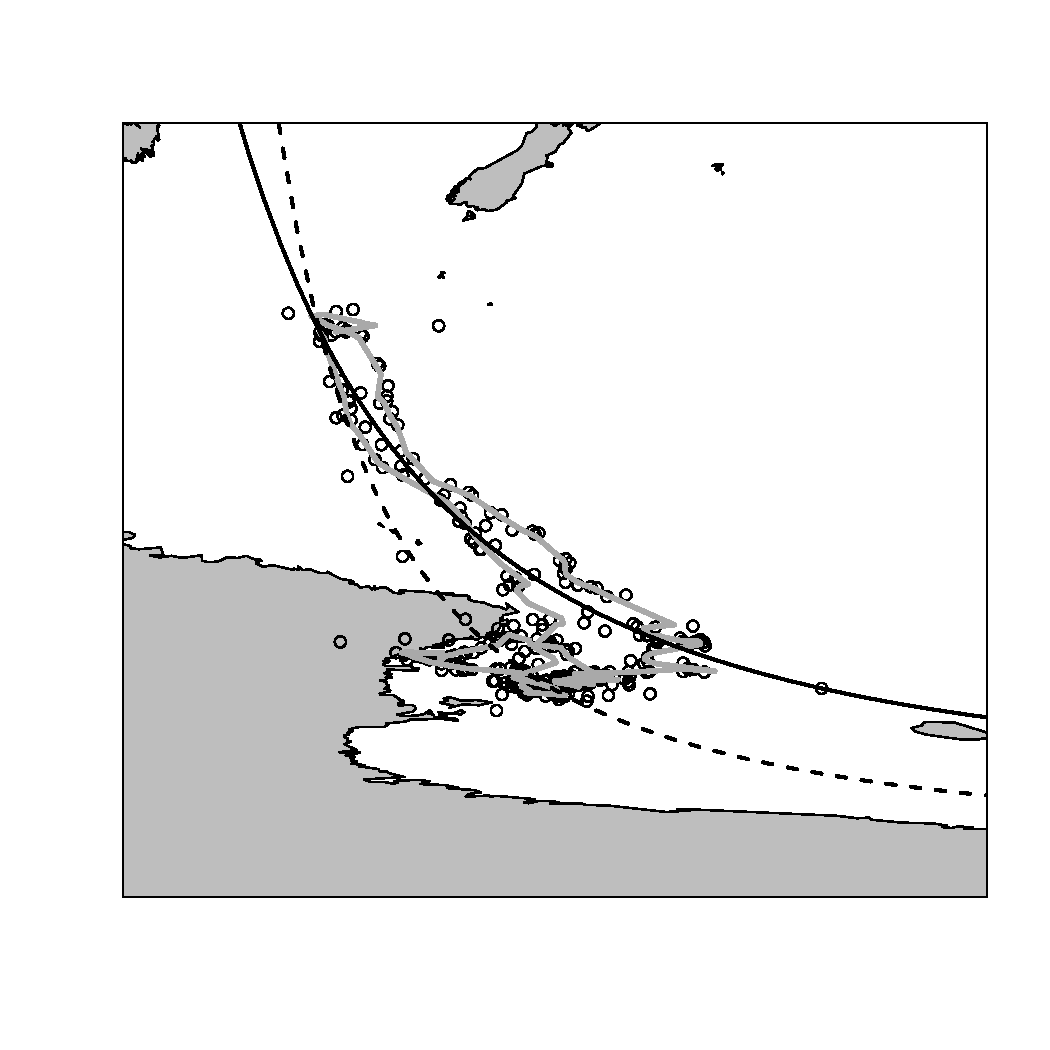
\includegraphics[width=\maxwidth]{figure/minimal-unnamed-chunk-9-1} 

}



\end{knitrout}
\end{center}
\caption{Raw Argos estimates and penalized smoothed track plotted in
  raw longitude and latitude. Great circles are drawn as curves, from
  Macquarie Island through the most distant raw Argos position (solid)
  and the most distant smooth position (dashed).}
\label{fig:LongLat}
\end{figure}

%% Make the point that the gc lines here aren't exactly straight, but
%% it's a much better choice because

Figure~\ref{fig:LongLat} shows that the perceived error in the Argos
positions in the east/west direction is far less and it is clear that
intuitive ideas about straight line travel are not easily conveyed in
longitude and latitude plots. The same data in Figure~\ref{fig:Proj}
uses a projection that more accurately represent great circles as
straight-lines.

\begin{figure}
\begin{center}
\begin{knitrout}
\definecolor{shadecolor}{rgb}{0.969, 0.969, 0.969}\color{fgcolor}

{\centering 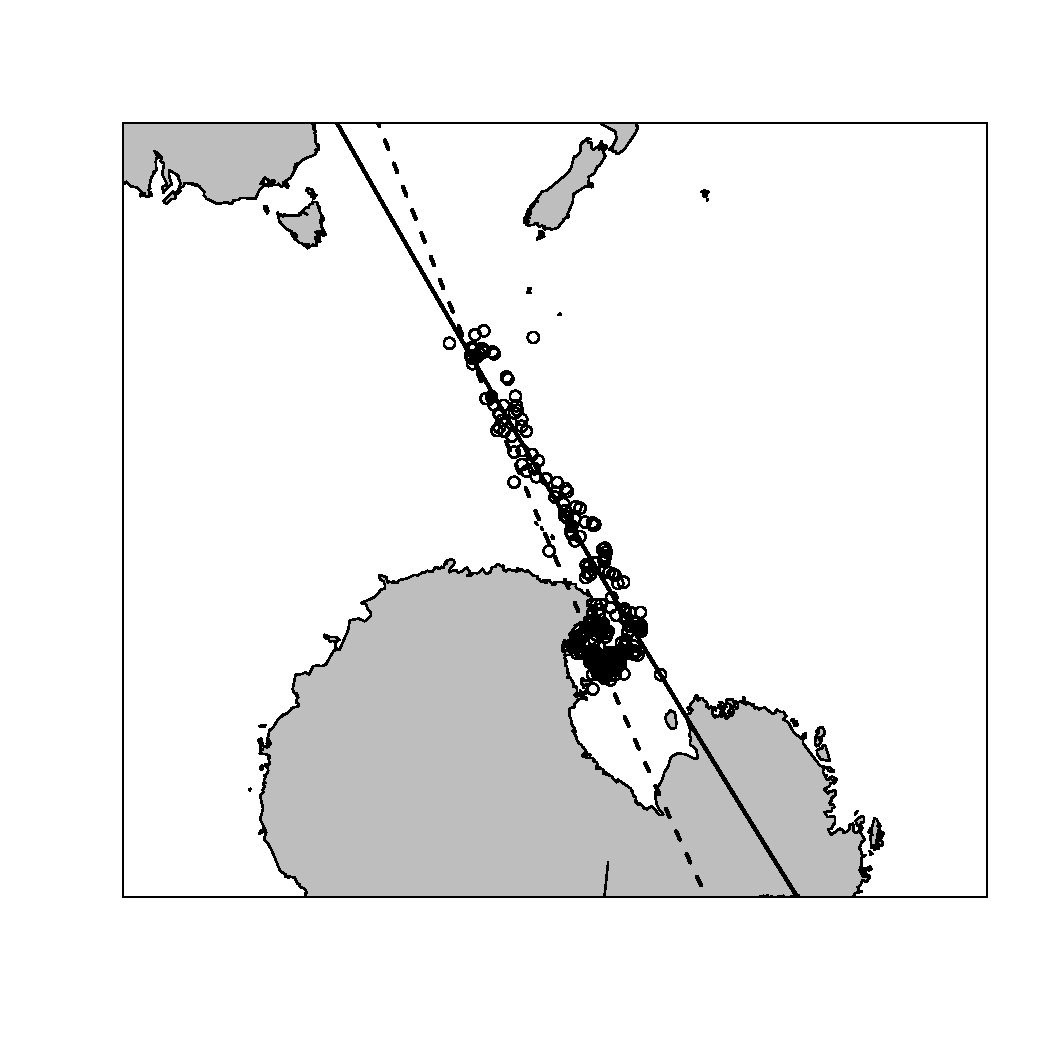
\includegraphics[width=\maxwidth]{figure/minimal-unnamed-chunk-10-1} 

}



\end{knitrout}
\end{center}
\caption{Raw Argos estimates and penalized smoothed track plotted in
  an equal-area projection. Great circles (as-the-crow-flies) are
  shown as lines. These pass through the Macquarie Island site to the
  most distant raw Argos position (solid) and the most distant smooth
  position (dashed).}
\label{fig:Proj}
\end{figure}



\subsection{Tools for traditional methods}
Given these limitations there is still a use for these filtering and
gridding methods. They are also used as part of more sophisticated
modelling approaches \citep{jonsen86rss,patterson2010using}. The
\pkg{trip} package provides a framework for running these algorithms
on sets of animal tracks within the validation requirements discussed
above. As it builds on the existing spatial infrastructure the package
provides simple access to arbitrary map projections and to input and
output for commonly used GIS vector and raster formats. Extra
capability is provided by linkages to the \pkg{raster} package to
simplify access to imagery, raster data and array formats like NetCDF
and to the \pkg{spatstat} package


% suite of tools trip, satin, manifR, msla, ...
%     - revisit each of the issues mentioned above, with examples using
%     trip
%     - then some more sophisticated subset/groups, overlay sat data

%     basic QA
%     subsetting, combining
%     visualization
%     analysis


\section{The trip package for animal track data}
\label{sec:tripdemo}

The \pkg{trip} package developed by the author provides programming
definitions and functions for working with animal track data in the
\proglang{R} programming environment. The package provides convenient
access to commonly used methods discussed in this chapter. The
\pkg{trip} package is available on \texttt{CRAN}:
\url{http://cran.r-project.org}\footnote{\pkg{Trip} replaced the
  experimental package \pkg{timeTrack} version 1.1-6, which provided
  similar functionality but was not integrated with \pkg{sp}.}.

The \pkg{trip} package builds on the spatial infrastructure of the
\pkg{sp} package. The \pkg{sp} package uses the S4 programming classes
and methods of \cite{chambers2008software} to provide a coherent system
for the usual spatial data types: points, lines, polygons and
grids. This system provides visualization and manipulation of
spatial data, a consistent conversion for data between the variety of
spatial statistics packages already in \proglang{R}, and interfaces to GIS and
map projections \citep{sp}. The following description of \pkg{sp} objects
given here is derived from \cite{sp} and \cite{asdar}, which should be
consulted for a more complete description.

All \pkg{sp} (and therefore \texttt{trip}) objects share the basic
property \texttt{Spatial} which stores only the bounding box and map
projection metadata. Each new data type then extends this to the variety
of spatial types with increasing specialization: coordinates and
levels of organization are added to provide \texttt{SpatialPoints},
\texttt{SpatialLines}, \texttt{SpatialPolygons} and
\texttt{SpatialGrids}. \texttt{Trip} objects are specializations of
the \texttt{SpatialPoints} class and so the other types are not
considered further here.

%% reviewed up to "separately"

The class \texttt{SpatialPoints} consists of a matrix of coordinates
and the \texttt{Spatial} metadata for their bounding box and map
projection---this is sufficient to locate each point on a map, but
applying more information for each point requires a matching attribute
table. For example data such as the name, size, colour, direction and
quality for each point may be stored as well as its location. The
basic table component in \proglang{R} is a \texttt{data.frame}, and
this is extended by the class \texttt{SpatialPointsDataFrame}. A
\texttt{SpatialPointsDataFrame} can be considered as a table of
records (a \texttt{data.frame}) containing X and Y coordinates and
other attributes. The coordinates are treated specially so that they
may be used to visualize or manipulate the object in a spatial
context\footnote{This is rather simple for points since there is only
  one coordinate for each record: the separation of coordinates and
  attribute data becomes important for more complicated spatial
  objects.}.  Objects of class \texttt{trip} extend this class
directly, by applying another level of information about the identity
of each trip, the temporal coordinate of each point and ensuring that
the records can be validated by the rules laid out in Section
\ref{sec:tripdef}. This is done with a new class
\texttt{TimeOrderedRecords} that stores the names of the date-time and
ID attribute in the records. Checks are applied for any object
aspiring to be of class \texttt{Spatial} and of class
\texttt{TimeOrderedRecords} by ensuring that time values are in order
within ID and that there are no duplicate times, no missing
coordinates etc. If any of these constraints is broken then validation
cannot occur and the object creation will fail. Further discussion and
illustration of the \texttt{trip} class definition in the context of
\pkg{sp} is given in \cite{asdar}.

By using the \pkg{sp} classes \pkg{trip} automatically gains all the
available methods for \texttt{Spatial} objects including plot, subset,
coordinate system metadata and reprojection, summary and print. A
\texttt{trip} object is considered as sets of ``TimeOrdered'' points,
rather than multi-segment lines. Some functions do assume
line-interpretion of trips, but in general the storage of attribute
data on ordered points provides greater flexibility than storage of
line objects for reasons discussed in Section~\ref{sec:software}.

The \pkg{trip} package depends entirely on the \pkg{methods} and
\pkg{sp} packages, and in part on the \pkg{spatstat} and
\pkg{maptools} packages \citep{spatstat,maptools}.


The next section demonstrates some examples using the \pkg{trip}
package for importing data, dealing with common problems and
``filtering'' and ``gridding'' track data.

\subsection{Generating trip objects}
\label{sec:generatetrip}
The following examples show the simplest means of generating a trip
object from a table of data. The function \texttt{readArgos} does all
of this internally, as shown below.  The \texttt{trip} class is derived
from classes in the package \pkg{sp} and so the first step is to
create a \texttt{SpatialPointsDataFrame}.

The following \proglang{R} code reads data from a text file, promotes
resulting table to a Spatial object and converts dates and times from
text.

\begin{knitrout}
\definecolor{shadecolor}{rgb}{0.969, 0.969, 0.969}\color{fgcolor}\begin{kframe}
\begin{alltt}
\hlcom{## originally this was the readArgos data, but now is this:}
\hlcom{## load("E:\textbackslash{}\textbackslash{}mike\textbackslash{}\textbackslash{}working\textbackslash{}\textbackslash{}doc\textbackslash{}\textbackslash{}PhD\textbackslash{}\textbackslash{}Thesis-MDSUMNER\textbackslash{}\textbackslash{}figuredata\textbackslash{}\textbackslash{}RawArgos.Rdata")}

\hlstd{dat} \hlkwb{<-} \hlkwd{read.csv}\hlstd{(}\hlstr{"trackfile.csv"}\hlstd{)}
\end{alltt}


{\ttfamily\noindent\bfseries\color{errorcolor}{\#\# Error in file(file, "{}rt"{}): cannot open the connection}}\begin{alltt}
\hlkwd{names}\hlstd{(dat)}  \hlcom{#[1] "long" "lat"  "seal"  "date"    "local"     "lq"}
\end{alltt}


{\ttfamily\noindent\bfseries\color{errorcolor}{\#\# Error in eval(expr, envir, enclos): object 'dat' not found}}\begin{alltt}
\hlkwd{library}\hlstd{(sp)}
\hlkwd{coordinates}\hlstd{(dat)} \hlkwb{<-} \hlkwd{c}\hlstd{(}\hlstr{"long"}\hlstd{,} \hlstr{"lat"}\hlstd{)}
\end{alltt}


{\ttfamily\noindent\bfseries\color{errorcolor}{\#\# Error in coordinates(dat) <- c("{}long"{}, "{}lat"{}): object 'dat' not found}}\begin{alltt}
\hlstd{dat}\hlopt{$}\hlstd{gmt} \hlkwb{<-} \hlkwd{as.POSIXct}\hlstd{(}\hlkwd{strptime}\hlstd{(}\hlkwd{paste}\hlstd{(dat}\hlopt{$}\hlstd{date, dat}\hlopt{$}\hlstd{local),}
                      \hlstr{"%d-%b-%y %H:%M:%S"}\hlstd{),} \hlkwc{tz} \hlstd{=} \hlstr{"GMT"}\hlstd{)} \hlopt{-} \hlnum{10} \hlopt{*} \hlnum{3600}
\end{alltt}


{\ttfamily\noindent\bfseries\color{errorcolor}{\#\# Error in paste(dat\$date, dat\$local): object 'dat' not found}}\end{kframe}
\end{knitrout}

A data frame in \proglang{R} is read in from text file using
\texttt{read.csv}. The column names are printed by the \texttt{names}
function. The \pkg{sp} function \texttt{coordinates} is used to
promote a data frame to a \texttt{Spatial} object by specifying which
columns contain the spatial coordinates.

The dates and times in this object are still just text from the file,
so these are converted to the \texttt{DateTimeClasses} provided by
\proglang{R}. An offset is applied to ensure the correct timezone
interpretation. The \texttt{strptime} function provides all the
required templates for parsing date-times from text---here the date
stamp is a parochial format with day, short month and short year.

The examples here use longitude and latitude data, but \texttt{trip}
objects can be generated using any valid coordinates. The projection
metadata may be stored as per the definition of the \texttt{Spatial}
classes in \pkg{sp}.

The following code attempts to generate a \texttt{trip} object by
assigning the time and ID attributes. This step often presents some
problems that need to be dealt with.

\begin{knitrout}
\definecolor{shadecolor}{rgb}{0.969, 0.969, 0.969}\color{fgcolor}\begin{kframe}
\begin{alltt}
\hlkwd{library}\hlstd{(trip)}
\end{alltt}
\end{kframe}
\end{knitrout}
\begin{knitrout}
\definecolor{shadecolor}{rgb}{0.969, 0.969, 0.969}\color{fgcolor}\begin{kframe}
\begin{alltt}
\hlstd{tr} \hlkwb{<-} \hlkwd{trip}\hlstd{(dat,} \hlkwd{c}\hlstd{(}\hlstr{"gmt"}\hlstd{,} \hlstr{"seal"}\hlstd{))}
\end{alltt}
\end{kframe}
\end{knitrout}
\begin{knitrout}
\definecolor{shadecolor}{rgb}{0.969, 0.969, 0.969}\color{fgcolor}\begin{kframe}
\begin{verbatim}
## Error in trip(dat, c("gmt", "seal")) : object 'dat' not found
## Error in trip(dat, c("gmt", "seal")) : object 'dat' not found
\end{verbatim}
\end{kframe}
\end{knitrout}

The \texttt{trip} function takes the \texttt{SpatialPointsDataFrame}
and the names of the date-time and ID columns. In this case the
attempt fails as the data will not validate in its current form. This
is important as it ensures that these simple problems are dealt with
upfront so they are not propagated further to cause problems in
subsequent analyses.

The next section shows an alternative method for reading \pkg{trip}
data from an Argos format.


\subsubsection{Reading data from Argos records}
\label{sec:readargos}
Argos (PRV/DAT) files can be read directly using the function
\texttt{readArgos} and if the defaults for basic quality control are
successful this will return a \texttt{trip} object.\footnote{These
  data were provided by the DPIWE Macquarie Island Albatross Project
  \citep{terauds2006foraging}.  Only three of the available Argos
  files are imported for this example.}



\begin{knitrout}
\definecolor{shadecolor}{rgb}{0.969, 0.969, 0.969}\color{fgcolor}\begin{kframe}
\begin{alltt}
\hlkwd{library}\hlstd{(trip)}
\hlcom{## read in some Argos data}
\hlstd{argosfiles} \hlkwb{<-} \hlkwd{list.files}\hlstd{(}\hlkwc{path} \hlstd{=} \hlstr{"G:/DATA/tracks/blackBrowed/"}\hlstd{,} \hlkwc{pattern} \hlstd{=} \hlstr{".dat"}\hlstd{,} \hlkwc{full.names} \hlstd{=} \hlnum{TRUE}\hlstd{,} \hlkwc{ignore.case} \hlstd{=} \hlnum{TRUE}\hlstd{)}
\hlstd{argosdata} \hlkwb{<-} \hlkwd{readArgos}\hlstd{(argosfiles[}\hlnum{1}\hlopt{:}\hlnum{3}\hlstd{])}
\end{alltt}


{\ttfamily\noindent\bfseries\color{errorcolor}{\#\# Error in file(con, "{}r"{}): cannot open the connection}}\begin{alltt}
\hlkwd{summary}\hlstd{(argosdata)}
\end{alltt}


{\ttfamily\noindent\bfseries\color{errorcolor}{\#\# Error in summary(argosdata): object 'argosdata' not found}}\end{kframe}
\end{knitrout}

%% depending on data used "Longitudes contain values greater than 180,
%% assuming proj.4 +over" - need to explain this?


In Argos PRV (DAT) files the fields \texttt{longitude} and \texttt{latitude}
contain the spatial coordinates (these have been extracted from the
other data in the \texttt{SpatialPointsDataFrame} in the usual way),
\texttt{date} and \texttt{time} the temporal information (these have
been combined into an \proglang{R} date-time column called
\texttt{gmt}), and \texttt{ptt} is the ID for individual instruments
that is used as the trip ID. The function \texttt{readArgos} will
perform some sensible quality control corrections by default. The
summary command returns a listing of the individual trips, their ID,
start and end times, and number of locations. The remaining data are
summarized in the usual way for a \pkg{SpatialPointsDataFrame}.

%The output in this example is a report on which records contained
%duplicate times, and have been modified slightly.

When reading data from PRV files the following coordinate system is
assumed:

\begin{center}
longitude / latitude on the WGS84 datum.
\end{center}

This is specified using the following \proglang{PROJ.4} string:
\begin{center}
\texttt{+proj=longlat +ellps=WGS84}.
\end{center}
If longitude values greater than 180 are present the ``+over'' element
is applied for the ``Pacific view [0,360]'' longitude convention. No
further checking is done.

The function \texttt{readDiag} reads Argos DIAG (diagnostic) format
that provides two sets of location coordinates. This function returns
a data frame with the attributes from the files.

\subsubsection{Dealing with common problems in track data} This
section begins with the raw data frame of track data from
\ref{sec:generatetrip}.
\begin{knitrout}
\definecolor{shadecolor}{rgb}{0.969, 0.969, 0.969}\color{fgcolor}\begin{kframe}
\begin{alltt}
\hlstd{dat} \hlkwb{<-} \hlkwd{as.data.frame}\hlstd{(dat)}
\end{alltt}


{\ttfamily\noindent\bfseries\color{errorcolor}{\#\# Error in as.data.frame(dat): object 'dat' not found}}\end{kframe}
\end{knitrout}

There are a number of simple problems at this stage that the
\texttt{trip} class automatically provides validation for. Duplicated
rows, such as those from overlapping Argos files, can be safely
dropped.

\begin{knitrout}
\definecolor{shadecolor}{rgb}{0.969, 0.969, 0.969}\color{fgcolor}\begin{kframe}
\begin{alltt}
\hlstd{dat} \hlkwb{<-} \hlstd{dat[}\hlopt{!}\hlkwd{duplicated}\hlstd{(dat), ]}
\end{alltt}


{\ttfamily\noindent\bfseries\color{errorcolor}{\#\# Error in eval(expr, envir, enclos): object 'dat' not found}}\begin{alltt}
\hlkwd{head}\hlstd{(dat)}
\end{alltt}


{\ttfamily\noindent\bfseries\color{errorcolor}{\#\# Error in head(dat): object 'dat' not found}}\end{kframe}
\end{knitrout}

The discarded rows removed are exact duplicate rows, matched on every
data value for each column.

The ordering of rows in the data is assumed to follow the order of the
date-time values with a trip ID. The date-time values are not used
automatically to order the data, as this could hide deeper problems in
a data set.

\begin{knitrout}
\definecolor{shadecolor}{rgb}{0.969, 0.969, 0.969}\color{fgcolor}\begin{kframe}
\begin{alltt}
\hlstd{dat} \hlkwb{<-} \hlstd{dat[}\hlkwd{order}\hlstd{(dat}\hlopt{$}\hlstd{seal, dat}\hlopt{$}\hlstd{gmt), ]}
\end{alltt}


{\ttfamily\noindent\bfseries\color{errorcolor}{\#\# Error in eval(expr, envir, enclos): object 'dat' not found}}\end{kframe}
\end{knitrout}

A final problem is that subsequent date-times within a single trip ID
can be duplicates. Removing duplicate rows and ordering the rows still
leaves the problem of what that can mean. If the location coordinates
are different, the implication is that the animal moved a certain
distance in no time at all. If the locations are the same then it begs
the question of why the tracking system distinguishes the records at
all. A zero duration time difference results in meaningless metrics of
speed of movement, for example. There is no obvious solution for this
and the issue must be investigated in the context of the actual data
used.  A simplistic solution that allows us to move on is to adjust
these duplicate times by a very small amount, so that the time
difference is not zero.
\begin{knitrout}
\definecolor{shadecolor}{rgb}{0.969, 0.969, 0.969}\color{fgcolor}\begin{kframe}
\begin{alltt}
\hlstd{dat}\hlopt{$}\hlstd{gmt} \hlkwb{<-} \hlkwd{adjust.duplicateTimes}\hlstd{(dat}\hlopt{$}\hlstd{gmt, dat}\hlopt{$}\hlstd{seal)}
\end{alltt}


{\ttfamily\noindent\bfseries\color{errorcolor}{\#\# Error in tapply(time, id, duplicated): object 'dat' not found}}\end{kframe}
\end{knitrout}

Further data problems are more fundamental and do not have easy
fixes. The \texttt{trip} class will fail to validate in the following
cases and these must be dealt with individually as appropriate.


\begin{description}
\item[Insufficient records for a given trip ID]Each set of records
  must have three or more locations to qualify as a \texttt{trip}. Sometimes
  the only available data is a start and end location but this case is
  deemed inappropriate for \pkg{trip}.
\item[Invalid values for critical data]Missing values or otherwise
  non-numeric values for locations and date-times cannot be
  included. The \pkg{sp} classes ensure this for location coordinates,
  and \texttt{trip} adds the limitation for date-times and IDs.
\item[Non-existent date and ID data]This is somewhat obvious, but \pkg{trip}
  will not assume a simple date-time value from the order of records
  or provide a default ID for single-trip data. These must be
  explicitly provided.
\end{description}

Once all of the fixes required have been applied, \texttt{trip}
validation is possible.

\begin{knitrout}
\definecolor{shadecolor}{rgb}{0.969, 0.969, 0.969}\color{fgcolor}\begin{kframe}
\begin{alltt}
\hlkwd{coordinates}\hlstd{(dat)} \hlkwb{<-} \hlkwd{c}\hlstd{(}\hlstr{"long"}\hlstd{,} \hlstr{"lat"}\hlstd{)}
\end{alltt}


{\ttfamily\noindent\bfseries\color{errorcolor}{\#\# Error in coordinates(dat) <- c("{}long"{}, "{}lat"{}): object 'dat' not found}}\begin{alltt}
\hlstd{tr} \hlkwb{<-} \hlkwd{trip}\hlstd{(dat,} \hlkwd{c}\hlstd{(}\hlstr{"gmt"}\hlstd{,} \hlstr{"seal"}\hlstd{))}
\end{alltt}


{\ttfamily\noindent\bfseries\color{errorcolor}{\#\# Error in trip(dat, c("{}gmt"{}, "{}seal"{})): object 'dat' not found}}\end{kframe}
\end{knitrout}

The location quality class is converted to an ordered factor, and the
appropriate \proglang{PROJ.4} string is applied.
\begin{knitrout}
\definecolor{shadecolor}{rgb}{0.969, 0.969, 0.969}\color{fgcolor}\begin{kframe}
\begin{alltt}
\hlstd{tr}\hlopt{$}\hlstd{class} \hlkwb{<-} \hlkwd{ordered}\hlstd{(tr}\hlopt{$}\hlstd{lq,} \hlkwd{c}\hlstd{(}\hlstr{"Z"}\hlstd{,} \hlstr{"B"}\hlstd{,} \hlstr{"A"}\hlstd{,} \hlstr{"0"}\hlstd{,} \hlstr{"1"}\hlstd{,} \hlstr{"2"}\hlstd{,} \hlstr{"3"}\hlstd{))}
\hlkwd{proj4string}\hlstd{(tr)} \hlkwb{<-} \hlkwd{CRS}\hlstd{(}\hlstr{"+proj=longlat +ellps=WGS84 +over"}\hlstd{)}
\end{alltt}
\end{kframe}
\end{knitrout}

The location quality class provided for Argos data is automatically
converted to an ``ordered factor'' by \texttt{readArgos}, here shown
manually. This can be used for simple selection of a range of records
from a data set, even though the tokens used as text have no inherent
order. This allows the data to be used directly without creating a
numeric proxy for the class values.


The resulting \texttt{trip} object read from CSV text is now validated
and equivalent to that returned by \texttt{readArgos}.


\subsection{Filtering for unlikely movement}

The infrastructure provided by the \pkg{trip} classes allows efficient
implementation of custom filters based on a variety of metrics.

The data are from southern elephant seals from Macquarie Island.
These animals can swim up to 12 km/hr \citep{BHMS02} so that value is
used to calculate a filter, which is added as a column in the data
frame. The filtering algorithm is that of \cite{MCF92}.

\begin{knitrout}
\definecolor{shadecolor}{rgb}{0.969, 0.969, 0.969}\color{fgcolor}\begin{kframe}
\begin{alltt}
\hlstd{tr}\hlopt{$}\hlstd{ok} \hlkwb{<-} \hlkwd{speedfilter}\hlstd{(tr,} \hlkwc{max.speed} \hlstd{=} \hlnum{12}\hlstd{)}
\hlkwd{summary}\hlstd{(tr)}
\end{alltt}
\begin{verbatim}
## 
## Object of class trip
##   tripID ("seal") No.Records   startTime ("gmt")     endTime ("gmt")  tripDuration
## 1            c026        351 1999-01-01 00:35:59 1999-05-21 15:29:17 140.6203 days
##   tripDistance meanSpeed maxSpeed meanRMSspeed maxRMSspeed
## 1     23490.23  120.4115 29332.07     119.2497    14666.07
## 
## Total trip duration: 12149598 seconds (3374 hours, 3198 seconds)
## 
## Derived from Spatial data:
## 
## Object of class SpatialPointsDataFrame
## Coordinates:
##            min       max
## long 156.46667 189.99167
## lat  -78.06333 -52.85667
## Is projected: FALSE 
## proj4string : [+proj=longlat +ellps=WGS84 +over]
## Number of points: 351
## Data attributes:
##    seal            date          local          gmt                      lq      class  
##  c026:351   27-Jan-99: 10   14:42:21:  2   Min.   :1999-01-01 11:35:59   0: 38   Z:  0  
##             17-Jan-99:  8   15:29:50:  2   1st Qu.:1999-01-30 01:28:14   1: 10   B:214  
##             14-Mar-99:  7   0:04:01 :  1   Median :1999-02-26 12:22:56   2:  8   A: 80  
##             15-Mar-99:  7   0:04:05 :  1   Mean   :1999-03-02 04:53:25   3:  1   0: 38  
##             28-Jan-99:  7   0:10:34 :  1   3rd Qu.:1999-03-27 01:44:51   A: 80   1: 10  
##             6-Feb-99 :  7   0:16:15 :  1   Max.   :1999-05-22 01:29:17   B:214   2:  8  
##             (Other)  :305   (Other) :343                                         3:  1  
##      ok         
##  Mode :logical  
##  FALSE:75       
##  TRUE :276      
##                 
##                 
##                 
## 
\end{verbatim}
\end{kframe}
\end{knitrout}

The \texttt{speedfilter} function assumes that speed is specified in
km/hr and distance is calculated based on the projection metadata. If
the projection is specified and not longitude and latitude then
Euclidean methods are applied. If the projection is not specified
longitude and latitude is assumed and ellipsoid methods for WGS84 are
used.

The summary shows that a number of locations are now classified by a
boolean value in a new ``ok'' column.  Although the speed filter has
not removed many locations, a customized subset can be defined based
on other data. Using a minimum Argos location quality class of
``A'' the raw data is plotted with a default point symbol and reduced
size, with lines connecting the remaining filtered points.  The plot
is shown in figure \ref{fig:pointsLines}.

%
%<<>>=
%plot(tr, axes = TRUE, cex = 0.4)
%lines(tr[tr$ok & tr$class > "B", ], lwd = 2, col = bpy.colors()[seq(10, 90, length = 4)])
%@

\begin{figure}
\begin{center}
\begin{knitrout}
\definecolor{shadecolor}{rgb}{0.969, 0.969, 0.969}\color{fgcolor}\begin{kframe}
\begin{alltt}
\hlkwd{plot}\hlstd{(tr,} \hlkwc{axes} \hlstd{=} \hlnum{TRUE}\hlstd{,} \hlkwc{cex} \hlstd{=} \hlnum{0.4}\hlstd{)}
\hlkwd{plot}\hlstd{(world,} \hlkwc{add} \hlstd{=} \hlnum{TRUE}\hlstd{,} \hlkwc{col} \hlstd{=} \hlstr{"grey"}\hlstd{)}
\hlkwd{lines}\hlstd{(tr[tr}\hlopt{$}\hlstd{ok} \hlopt{&} \hlstd{tr}\hlopt{$}\hlstd{class} \hlopt{>} \hlstr{"B"}\hlstd{, ],} \hlkwc{lwd} \hlstd{=} \hlnum{2}\hlstd{,}
      \hlkwc{col} \hlstd{=} \hlkwd{bpy.colors}\hlstd{()[}\hlkwd{seq}\hlstd{(}\hlnum{10}\hlstd{,} \hlnum{90}\hlstd{,} \hlkwc{length} \hlstd{=} \hlnum{4}\hlstd{)])}
\end{alltt}
\end{kframe}

{\centering 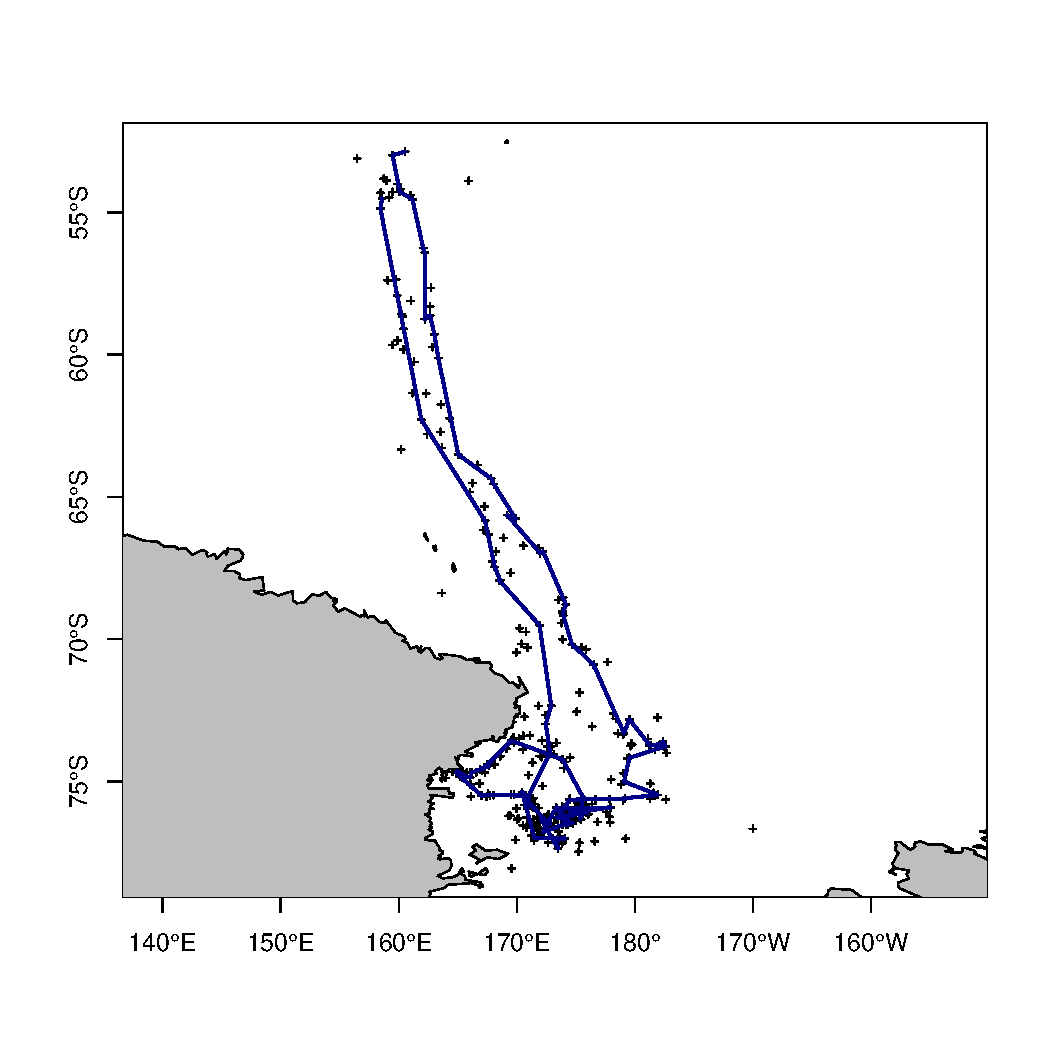
\includegraphics[width=\maxwidth]{figure/minimal-unnamed-chunk-23-1} 

}



\end{knitrout}
\end{center}
\caption{Plot of trips as points, with lines coloured for each separate
  trip.}
\label{fig:pointsLines}
\end{figure}

If this were calculated with coordinates in a different unit or
projection the \texttt{speedfilter} function takes this into account
and calculates distance accordingly. This integration of spatial
metadata and calculation provides for a very flexible working
environment for exploratory analysis.

\subsubsection{Extending the trip package}
\label{sec:extendingtrip}
One of the advantages of the infrastructure provided by the trip
classes is that simple tasks can be strung together efficiently. This
example shows how the speed-distance-angle filter of
\cite{freitas2008simple} can be built up from the basic tool kit.

The speed distance angle filter is distributed with an easily run
example, as follows. This is reproduced almost exactly from the
documentation for \texttt{argosfilter} in \cite{argosfilter}.


\begin{knitrout}
\definecolor{shadecolor}{rgb}{0.969, 0.969, 0.969}\color{fgcolor}\begin{kframe}
\begin{alltt}
\hlkwd{library}\hlstd{(argosfilter)}
\hlkwd{data}\hlstd{(seal)}
\hlstd{lat} \hlkwb{<-} \hlstd{seal}\hlopt{$}\hlstd{lat}
\hlstd{lon} \hlkwb{<-} \hlstd{seal}\hlopt{$}\hlstd{lon}
\hlstd{dtime} \hlkwb{<-} \hlstd{seal}\hlopt{$}\hlstd{dtime}
\hlstd{lc} \hlkwb{<-} \hlstd{seal}\hlopt{$}\hlstd{lc}
\hlstd{cfilter} \hlkwb{<-} \hlkwd{sdafilter}\hlstd{(lat, lon, dtime, lc)}

\hlstd{seal}\hlopt{$}\hlstd{sda} \hlkwb{<-} \hlopt{!}\hlstd{(cfilter} \hlopt{==} \hlstr{"removed"}\hlstd{)}
\end{alltt}
\end{kframe}
\end{knitrout}

This filter results in a column of values that specify whether the
filter retains or discards the location. The following steps create a
new version of this filter using the \pkg{trip} package. Load the
example data and validate as a single event trip object.
\begin{knitrout}
\definecolor{shadecolor}{rgb}{0.969, 0.969, 0.969}\color{fgcolor}\begin{kframe}
\begin{alltt}
\hlkwd{library}\hlstd{(argosfilter)}
\hlkwd{library}\hlstd{(sp)}
\hlkwd{library}\hlstd{(trip)}
\hlkwd{library}\hlstd{(maptools)}

\hlstd{trackAngle} \hlkwb{<-} \hlkwa{function}\hlstd{(}\hlkwc{xy}\hlstd{) \{}
    \hlstd{angles} \hlkwb{<-} \hlkwd{abs}\hlstd{(}\hlkwd{c}\hlstd{(}\hlkwd{trackAzimuth}\hlstd{(xy),} \hlnum{0}\hlstd{)} \hlopt{-}
                  \hlkwd{c}\hlstd{(}\hlnum{0}\hlstd{,} \hlkwd{rev}\hlstd{(}\hlkwd{trackAzimuth}\hlstd{(xy[}\hlkwd{nrow}\hlstd{(xy)}\hlopt{:}\hlnum{1}\hlstd{, ]))))}
    \hlstd{angles} \hlkwb{<-} \hlkwd{ifelse}\hlstd{(angles} \hlopt{>} \hlnum{180}\hlstd{,} \hlnum{360} \hlopt{-} \hlstd{angles, angles)}
    \hlstd{angles[}\hlkwd{is.na}\hlstd{(angles)]} \hlkwb{<-} \hlnum{180}
    \hlstd{angles}
\hlstd{\}}


\hlcom{## default values used by sdafilter}
\hlstd{vmax} \hlkwb{<-}  \hlnum{2}
\hlstd{ang} \hlkwb{<-} \hlkwd{c}\hlstd{(}\hlnum{15}\hlstd{,} \hlnum{25}\hlstd{)}
\hlstd{distlim} \hlkwb{<-} \hlkwd{c}\hlstd{(}\hlnum{2500}\hlstd{,}\hlnum{5000}\hlstd{)}


\hlkwd{coordinates}\hlstd{(seal)} \hlkwb{<-} \hlopt{~}\hlstd{lon}\hlopt{+}\hlstd{lat}
\hlkwd{proj4string}\hlstd{(seal)} \hlkwb{<-} \hlkwd{CRS}\hlstd{(}\hlstr{"+proj=longlat +ellps=WGS84"}\hlstd{)}
\hlstd{seal}\hlopt{$}\hlstd{id} \hlkwb{<-} \hlstr{"seal"}
\end{alltt}
\end{kframe}
\end{knitrout}

Perform some simple sanity checks before proceeding.
\begin{knitrout}
\definecolor{shadecolor}{rgb}{0.969, 0.969, 0.969}\color{fgcolor}\begin{kframe}
\begin{alltt}
\hlkwd{range}\hlstd{(}\hlkwd{diff}\hlstd{(seal}\hlopt{$}\hlstd{dtime))}
\end{alltt}
\begin{verbatim}
## Time differences in secs
## [1]      0 362737
\end{verbatim}
\begin{alltt}
\hlkwd{which}\hlstd{(}\hlkwd{duplicated}\hlstd{(seal}\hlopt{$}\hlstd{dtime))}
\end{alltt}
\begin{verbatim}
## [1]   18  117  123 1009 1159 1232 1294 1301
\end{verbatim}
\end{kframe}
\end{knitrout}

There are some preliminary requirements to load packages and
functions for earth distances and track turning angles. The
\texttt{seal} object is a data frame with columns ``lon'', ``lat'',
``dtime'' and ``lc''. The date-time values are already in
\texttt{POSIXct} format, and lc uses a numeric code for the Argos
class.

The records are in order of date-time, but some of the date-time
values are duplicated, so for illustration these are dropped and
then a new \texttt{trip} object is created.
%``Z''
\begin{knitrout}
\definecolor{shadecolor}{rgb}{0.969, 0.969, 0.969}\color{fgcolor}\begin{kframe}
\begin{alltt}
\hlstd{seal} \hlkwb{<-} \hlstd{seal[}\hlopt{!}\hlkwd{duplicated}\hlstd{(seal}\hlopt{$}\hlstd{dtime), ]}

\hlstd{seal.tr} \hlkwb{<-} \hlkwd{trip}\hlstd{(seal,} \hlkwd{c}\hlstd{(}\hlstr{"dtime"}\hlstd{,} \hlstr{"id"}\hlstd{))}
\end{alltt}
\end{kframe}
\end{knitrout}

First, add the filter from the \texttt{sdafilter} function to the trip
object, and also the basic speed filter available in the \pkg{trip}
package (using km/hr rather than m/s).

\begin{knitrout}
\definecolor{shadecolor}{rgb}{0.969, 0.969, 0.969}\color{fgcolor}\begin{kframe}
\begin{alltt}
\hlstd{seal.tr}\hlopt{$}\hlstd{speed.ok} \hlkwb{<-} \hlkwd{speedfilter}\hlstd{(seal.tr,} \hlkwc{max.speed} \hlstd{= vmax} \hlopt{*} \hlnum{3.6}\hlstd{)}
\end{alltt}
\end{kframe}
\end{knitrout}

Perform the initial simple processing for the speed distance angle
filter.

\begin{knitrout}
\definecolor{shadecolor}{rgb}{0.969, 0.969, 0.969}\color{fgcolor}\begin{kframe}
\begin{alltt}
\hlcom{## distances in metres}
\hlstd{dsts} \hlkwb{<-} \hlkwd{trackDistance}\hlstd{(}\hlkwd{coordinates}\hlstd{(seal.tr))} \hlopt{*} \hlnum{1000}
\hlstd{angs} \hlkwb{<-} \hlkwd{trackAngle}\hlstd{(}\hlkwd{coordinates}\hlstd{(seal.tr))}

\hlstd{dprev} \hlkwb{<-} \hlkwd{c}\hlstd{(}\hlnum{0}\hlstd{, dsts)}
\hlstd{dnext} \hlkwb{<-} \hlkwd{c}\hlstd{(dsts,} \hlnum{0}\hlstd{)}

\hlcom{## speed, lc, max distance}
\hlstd{ok} \hlkwb{<-} \hlstd{(seal.tr}\hlopt{$}\hlstd{speed.ok} \hlopt{|} \hlstd{dprev} \hlopt{<=} \hlnum{5000}\hlstd{)} \hlopt{&}  \hlstd{(seal.tr}\hlopt{$}\hlstd{lc} \hlopt{> -}\hlnum{9}\hlstd{)}
\end{alltt}
\end{kframe}
\end{knitrout}

This creates a logical vector where the speedfilter and
distance-previous pass, and discard any location class of ``Z'' (coded
as ``-9'' in this example). This is effectively the first pass of the
filter, distinguishing distance previous and distance next for each
point.

Now the remaining parts of the filter can be run---testing for angle
and distance combinations over the specified limit.  Some
housekeeping---create an index to keep track while running the filter on the
two distance/angle limits. A temporary copy of the \texttt{trip} is used to
make matching the filter easy as points are removed.

\begin{knitrout}
\definecolor{shadecolor}{rgb}{0.969, 0.969, 0.969}\color{fgcolor}\begin{kframe}
\begin{alltt}
\hlstd{seal.tr}\hlopt{$}\hlstd{filt.row} \hlkwb{<-} \hlnum{1}\hlopt{:}\hlkwd{nrow}\hlstd{(seal.tr)}
\hlstd{seal.tr}\hlopt{$}\hlstd{ok} \hlkwb{<-} \hlkwd{rep}\hlstd{(}\hlnum{FALSE}\hlstd{,} \hlkwd{nrow}\hlstd{(seal.tr))}

\hlstd{df} \hlkwb{<-} \hlstd{seal.tr}

\hlcom{## first subset}
\hlstd{df} \hlkwb{<-} \hlstd{df[ok, ]}
\hlcom{## distlim and angles, progressively}
\hlkwa{for} \hlstd{(i} \hlkwa{in} \hlnum{1}\hlopt{:}\hlkwd{length}\hlstd{(distlim)) \{}
    \hlstd{dsts} \hlkwb{<-} \hlkwd{trackDistance}\hlstd{(}\hlkwd{coordinates}\hlstd{(df))} \hlopt{*} \hlnum{1000}
    \hlstd{angs} \hlkwb{<-} \hlkwd{trackAngle}\hlstd{(}\hlkwd{coordinates}\hlstd{(df))}
    \hlstd{dprev} \hlkwb{<-} \hlkwd{c}\hlstd{(}\hlnum{0}\hlstd{, dsts)}
    \hlstd{dnext} \hlkwb{<-} \hlkwd{c}\hlstd{(dsts,} \hlnum{0}\hlstd{)}
    \hlstd{ok} \hlkwb{<-} \hlstd{(dprev} \hlopt{<=} \hlstd{distlim[i]} \hlopt{|} \hlstd{dnext} \hlopt{<=} \hlstd{distlim[i])}  \hlopt{|} \hlstd{angs} \hlopt{>} \hlstd{ang[i]}
    \hlstd{ok[}\hlkwd{c}\hlstd{(}\hlnum{1}\hlopt{:}\hlnum{2}\hlstd{, (}\hlkwd{length}\hlstd{(ok)}\hlopt{-}\hlnum{1}\hlstd{)}\hlopt{:}\hlkwd{length}\hlstd{(ok))]} \hlkwb{<-} \hlnum{TRUE}
    \hlstd{df} \hlkwb{<-} \hlstd{df[ok, ]}
    \hlstd{ok} \hlkwb{<-} \hlkwd{rep}\hlstd{(}\hlnum{TRUE}\hlstd{,} \hlkwd{nrow}\hlstd{(df))}
\hlstd{\}}
\end{alltt}
\end{kframe}
\end{knitrout}

The result is now a reduced \texttt{trip} with missing rows discarded by the
filter. Using the row index created earlier, match the filter result to
the original rows and tabulate the filter values for the original
sdafilter and the trip version. The number of accepted points is
nearly the same.

\begin{knitrout}
\definecolor{shadecolor}{rgb}{0.969, 0.969, 0.969}\color{fgcolor}\begin{kframe}
\begin{alltt}
\hlstd{seal.tr}\hlopt{$}\hlstd{ok[} \hlkwd{match}\hlstd{(df}\hlopt{$}\hlstd{filt.row, seal.tr}\hlopt{$}\hlstd{filt.row)]} \hlkwb{<-} \hlstd{ok}

\hlkwd{sum}\hlstd{(seal.tr}\hlopt{$}\hlstd{sda)}
\end{alltt}
\begin{verbatim}
## [1] 1135
\end{verbatim}
\begin{alltt}
\hlkwd{table}\hlstd{(seal.tr}\hlopt{$}\hlstd{sda, seal.tr}\hlopt{$}\hlstd{lc)}
\end{alltt}
\begin{verbatim}
##        
##          -9  -2  -1   0   1   2   3
##   FALSE  26 302  48  17  17   6   2
##   TRUE    0 374 374  61 150 116  60
\end{verbatim}
\begin{alltt}
\hlkwd{sum}\hlstd{(seal.tr}\hlopt{$}\hlstd{ok)}
\end{alltt}
\begin{verbatim}
## [1] 694
\end{verbatim}
\begin{alltt}
\hlkwd{table}\hlstd{(seal.tr}\hlopt{$}\hlstd{ok, seal.tr}\hlopt{$}\hlstd{lc)}
\end{alltt}
\begin{verbatim}
##        
##          -9  -2  -1   0   1   2   3
##   FALSE  26 482 185  38  65  46  17
##   TRUE    0 194 237  40 102  76  45
\end{verbatim}
\end{kframe}
\end{knitrout}

Plot the result to see that the new \pkg{trip} version is comparable. There
are differences since the distance and angle calculations are
ellipsoid based, rather than spherical as used by \pkg{argosfilter}
and some locations were first discarded due to impossible duplicate
times in the original data. There are probably also differences in the
detail of the recursive speed filter and the way that peaks are
assessed.

\begin{figure}
\begin{center}
\begin{knitrout}
\definecolor{shadecolor}{rgb}{0.969, 0.969, 0.969}\color{fgcolor}

{\centering 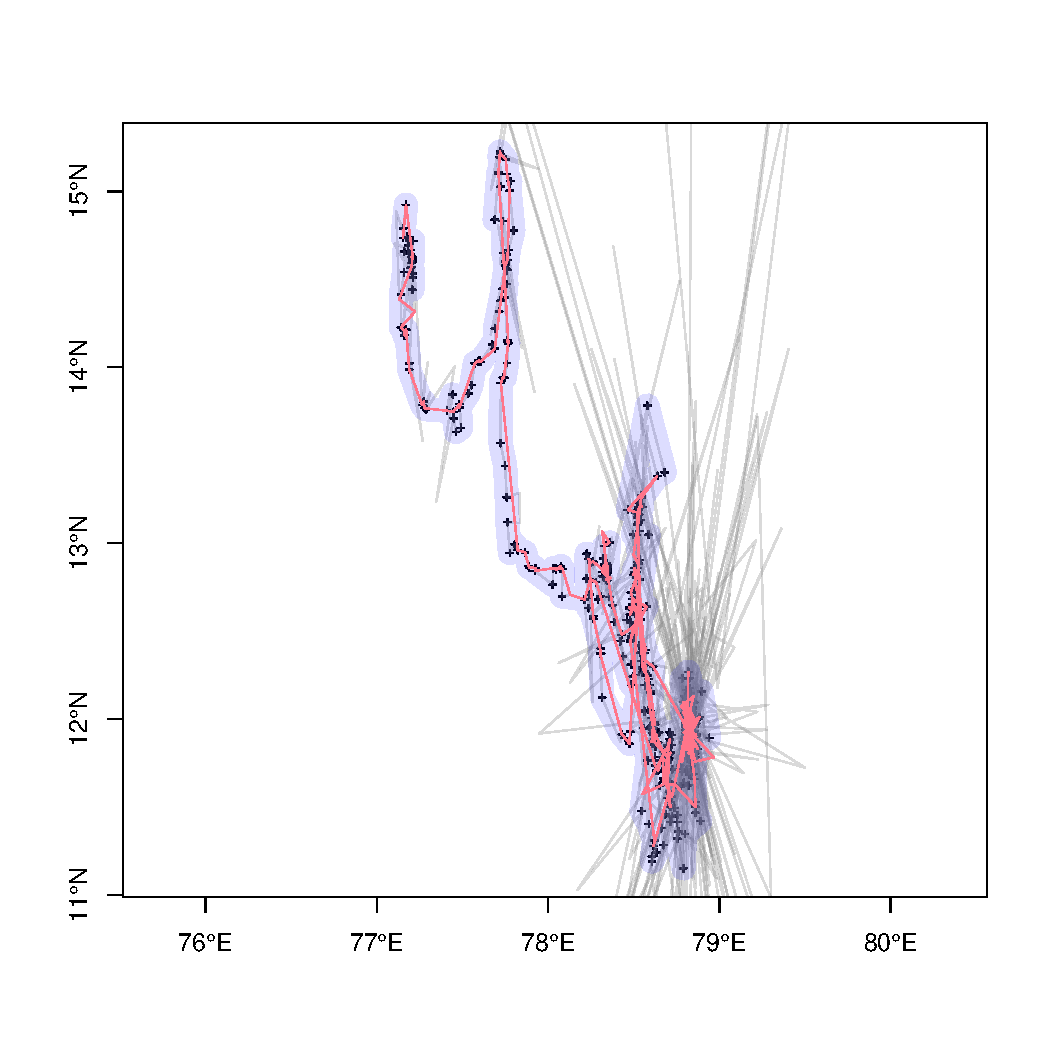
\includegraphics[width=\maxwidth]{figure/minimal-unnamed-chunk-33-1} 

}



\end{knitrout}
\end{center}
\caption{Original \texttt{sdafilter} (red) and custom \pkg{trip} speed
  distance angle filter (thick grey line). The original raw track is
  shown as a thin grey line.  }
\label{fig:customsda}
\end{figure}

The examples above consist of a working prototype that can be wrapped
as a function for the \pkg{trip} package to efficiently apply this
filter to sets of tracks within a \texttt{trip} object. The
\pkg{argosfilter} example above takes at least three times as long to
complete as the code developed above. The ability to extend the
functionality in this way mirrors the development of the \pkg{trip}
package itself, from the \pkg{sp} package, and in turn the
\proglang{R} platform.

\subsection{Creating maps of time spent}
Assuming that the filtered locations give realistic information about
position for the animal and that motion between these positions is
constant and straight, a map of time spent, or residency can be
created.  The choice of grid cell size might reflect the confidence in
the accuracy of the location data, or require a specific cell size for
comparison with another data set.

Using the trip locations accepted by the speed filter attribute
generate a grid of time spent, shown in Figure~\ref{fig:simplegrid}.

 %% load it to avoid the chatter



\begin{figure}
  \begin{center}
\begin{knitrout}
\definecolor{shadecolor}{rgb}{0.969, 0.969, 0.969}\color{fgcolor}\begin{kframe}
\begin{alltt}
\hlstd{trg}  \hlkwb{<-} \hlkwd{tripGrid}\hlstd{(tr[tr}\hlopt{$}\hlstd{ok, ])}
\hlkwd{image}\hlstd{(trg,} \hlkwc{col} \hlstd{=} \hlkwd{oc.colors}\hlstd{(}\hlnum{100}\hlstd{),} \hlkwc{axes} \hlstd{=} \hlnum{TRUE}\hlstd{)}
\end{alltt}
\end{kframe}

{\centering 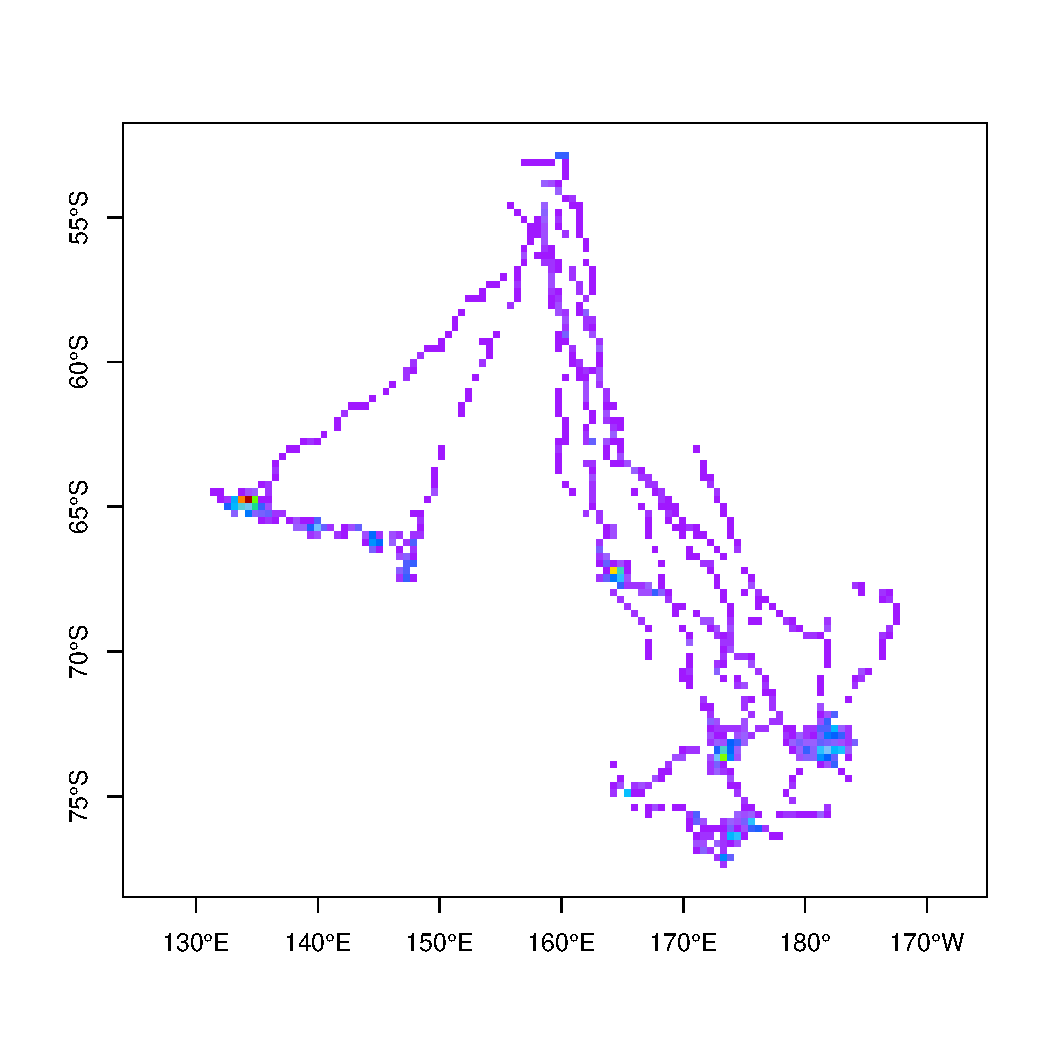
\includegraphics[width=\maxwidth]{figure/minimal-unnamed-chunk-35-1} 

}



\end{knitrout}
\end{center}
\caption{Simple image of a time spent grid for the trip object.}
\label{fig:simplegrid}
\end{figure}


%% transparent colours for image overlay on lines (maybe)
%t.cols <- col2rgb(oc.colors(256))
%t.cols <- rgb(t.cols[1,], t.cols[2,], t.cols[3,], 150, maxColorValue = 255)

%Running the algorithm used for \texttt{tripGrid} requires the
%\pkg{spatstat} package must be installed but will be loaded
%automatically.
The function \texttt{tripGrid} is used with the subset of the trip
object accepted by the speed filter to create a grid of time
spent. The algorithm used cuts the line segments exactly as described
in section \ref{sec:exactgridding} by the \pkg{spatstat} function
\texttt{pixellate}. If any zero-length line segments are present a
warning is issued and their time contribution is included as
points. This is because the pixellate algorithm relies on weightings
that are relative to the line length, which is another example of the
subtle implications of point versus line interpretations.

The gridded object \texttt{trg} is a \texttt{SpatialGridDataFrame},
whose class definition is provided by the \texttt{sp} package. These
grids support multiple attributes and so, conveniently, variations on
the map created can be stored in a single object.

Add three new attributes to the grid object by isolating a single
animal's trip, and using the kernel density method with two different
sigma values.

\begin{knitrout}
\definecolor{shadecolor}{rgb}{0.969, 0.969, 0.969}\color{fgcolor}\begin{kframe}
\begin{alltt}
\hlkwd{names}\hlstd{(trg)} \hlkwb{<-} \hlstr{'grid.filtered'}
\hlstd{gt} \hlkwb{<-} \hlkwd{getGridTopology}\hlstd{(trg)}
\hlstd{trg}\hlopt{$}\hlstd{grid.c026}  \hlkwb{<-} \hlkwd{tripGrid}\hlstd{(tr[tr}\hlopt{$}\hlstd{ok} \hlopt{&} \hlstd{tr}\hlopt{$}\hlstd{seal} \hlopt{==} \hlstr{"c026"}\hlstd{, ],} \hlkwc{grid} \hlstd{= gt)}\hlopt{$}\hlstd{z}
\hlstd{trg}\hlopt{$}\hlstd{kde1.filtered} \hlkwb{<-} \hlkwd{tripGrid}\hlstd{(tr[tr}\hlopt{$}\hlstd{ok, ],} \hlkwc{grid} \hlstd{= gt,} \hlkwc{method} \hlstd{=} \hlstr{"density"}\hlstd{,} \hlkwc{sigma} \hlstd{=} \hlnum{0.1}\hlstd{)}\hlopt{$}\hlstd{z}
\hlstd{trg}\hlopt{$}\hlstd{kde3.filtered} \hlkwb{<-} \hlkwd{tripGrid}\hlstd{(tr[tr}\hlopt{$}\hlstd{ok, ],} \hlkwc{grid} \hlstd{= gt,} \hlkwc{method} \hlstd{=} \hlstr{"density"}\hlstd{,} \hlkwc{sigma} \hlstd{=} \hlnum{0.3}\hlstd{)}\hlopt{$}\hlstd{z}

\hlkwa{for} \hlstd{(col.name} \hlkwa{in} \hlkwd{names}\hlstd{(trg)) trg[[col.name]]} \hlkwb{<-} \hlstd{trg[[col.name]]}\hlopt{/}\hlnum{3600}
\end{alltt}
\end{kframe}
\end{knitrout}

\begin{figure}
\begin{center}




\begin{knitrout}
\definecolor{shadecolor}{rgb}{0.969, 0.969, 0.969}\color{fgcolor}\begin{kframe}
\begin{alltt}
\hlkwd{require}\hlstd{(lattice)}
\hlkwd{library}\hlstd{(trip)}
\hlkwd{trellis.par.set}\hlstd{(}\hlstr{"regions"}\hlstd{,} \hlkwd{list}\hlstd{(}\hlkwc{col}\hlstd{=}\hlkwd{oc.colors}\hlstd{(}\hlnum{256}\hlstd{)))}
\hlkwd{print}\hlstd{(} \hlkwd{spplot}\hlstd{(trg))}
\end{alltt}
\end{kframe}

{\centering 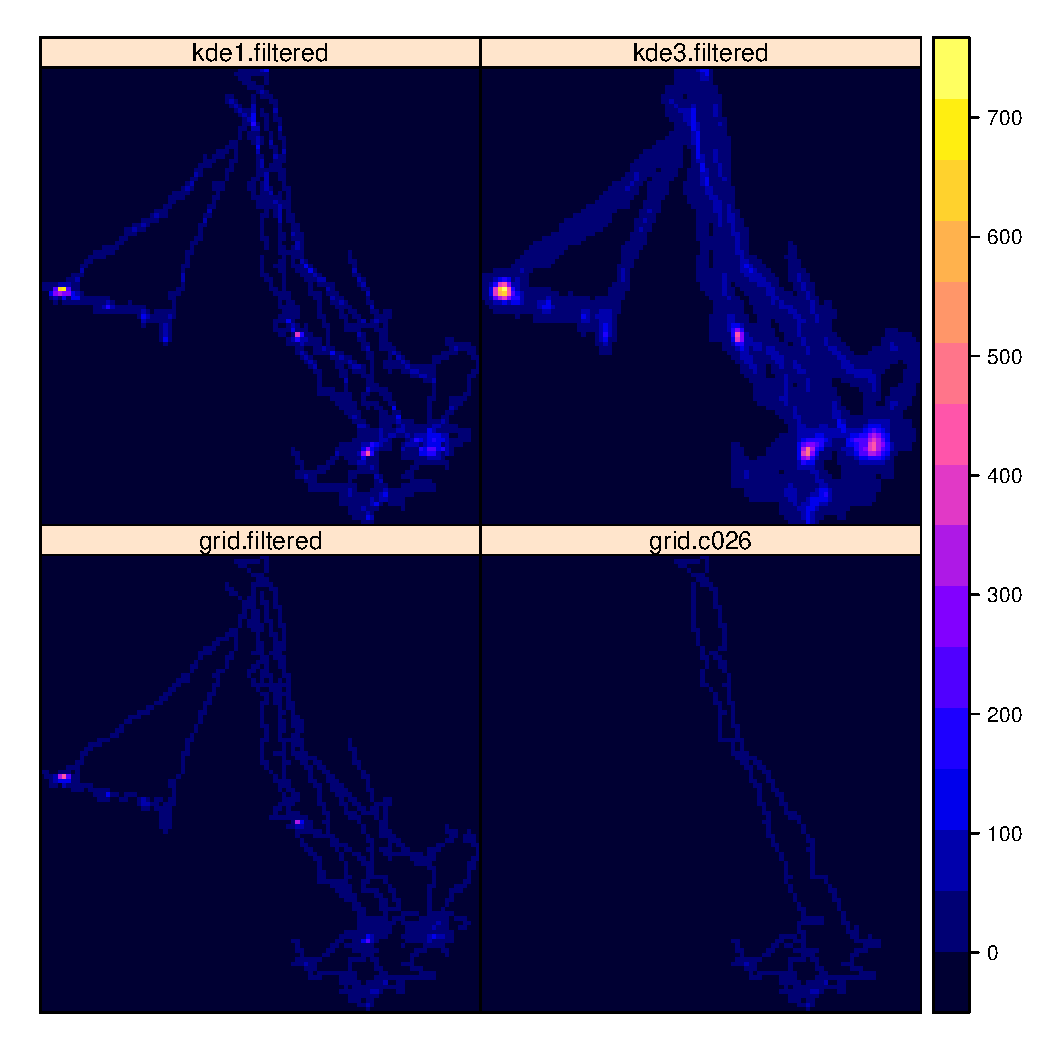
\includegraphics[width=\maxwidth]{figure/minimal-unnamed-chunk-38-1} 

}



\end{knitrout}
\end{center}
\caption{Four variations on a tripGrid. \texttt{grid.filtered} and
  \texttt{grid.c026} use the simple line-in-cell method for all four
  seals and for seal c026 alone. \texttt{kde3.filtered} and
  \texttt{kde1.filtered} use the kernel density method for line
  segments with a sigma of 0.3 and 0.1 respectively. Each grid has
  dimensions 100x100 and time spent is presented in hours.}
 \label{fig:fourgrids}
\end{figure}


The default name for an attribute from \texttt{tripGrid} is ``z'' so
first this is renamed to ``grid.filtered''. Calculation for the extra
attributes requires that they share the same origin and scale so this
is stored in the \texttt{GridTopology} object \texttt{gt} and used
again. The \texttt{trip} object is subset on the speed filter attribute and the
seal ID, and the resulting grid attribute ``z'' is extracted and
assigned to the grid object in one step. For the kernel density
versions two values of sigma are passed onto the \texttt{density}
function for each grid. The default output is in seconds, so this is
converted to hours for each grid column by division. Finally, the
multi-panel \texttt{spplot} function in package \texttt{sp} provides a
conveniently scaled image for each of the four grids shown in
Figure~\ref{fig:fourgrids}.


By default, \texttt{tripGrid} will provide a grid with dimensions
100x100 cells. This can be controlled exactly using a
\texttt{GridTopology} passed in as the grid argument to the function.
The convenience function \texttt{makeGridTopology} allows the user to
define a specific grid from the trip object itself.


The next examples use \texttt{trip} object to create grids with a
different scale.


\begin{knitrout}
\definecolor{shadecolor}{rgb}{0.969, 0.969, 0.969}\color{fgcolor}

{\centering 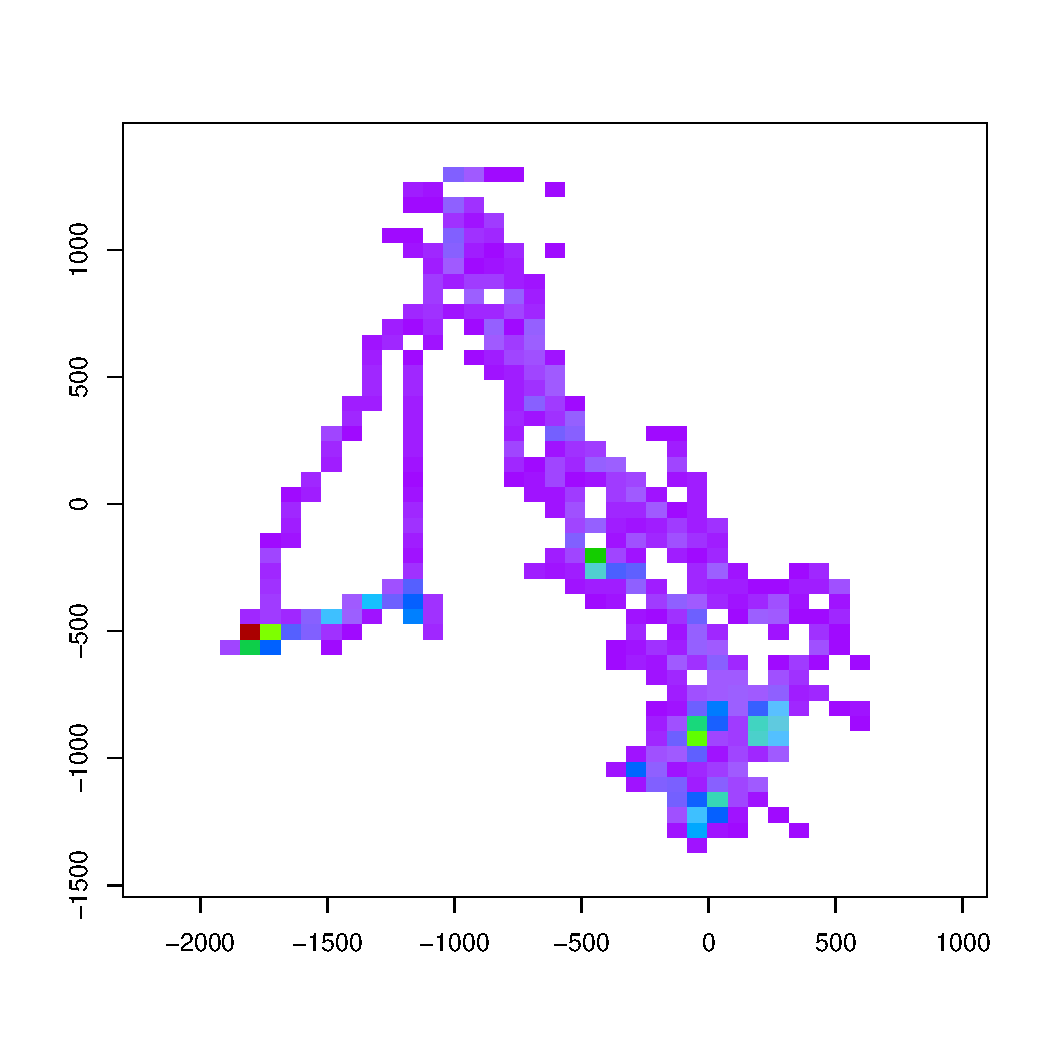
\includegraphics[width=\maxwidth]{figure/minimal-unnamed-chunk-39-1} 

}



\end{knitrout}

\begin{figure}
  \begin{center}
\begin{knitrout}
\definecolor{shadecolor}{rgb}{0.969, 0.969, 0.969}\color{fgcolor}\begin{kframe}
\begin{alltt}
\hlkwd{proj4string}\hlstd{(tr)} \hlkwb{<-} \hlkwd{CRS}\hlstd{(}\hlstr{"+proj=longlat +ellps=WGS84"}\hlstd{)}
\hlstd{p4} \hlkwb{<-} \hlkwd{CRS}\hlstd{(}\hlstr{"+proj=laea +lon_0=174.5 +lat_0=-65.5 +units=km"}\hlstd{)}

\hlstd{ptr} \hlkwb{<-} \hlkwd{tripTransform}\hlstd{(tr, p4)}

\hlstd{gt} \hlkwb{<-} \hlkwd{makeGridTopology}\hlstd{(ptr,} \hlkwd{c}\hlstd{(}\hlnum{50}\hlstd{,} \hlnum{50}\hlstd{))}
\hlstd{gt1} \hlkwb{<-} \hlkwd{makeGridTopology}\hlstd{(ptr,} \hlkwc{cellsize} \hlstd{=} \hlkwd{c}\hlstd{(}\hlnum{80}\hlstd{,} \hlnum{60}\hlstd{))}

\hlstd{grd2} \hlkwb{<-} \hlkwd{tripGrid}\hlstd{(ptr,} \hlkwc{grid} \hlstd{= gt1)}
\hlkwd{image}\hlstd{(grd2,} \hlkwc{col} \hlstd{=} \hlkwd{oc.colors}\hlstd{(}\hlnum{256}\hlstd{),} \hlkwc{axes} \hlstd{=} \hlnum{TRUE}\hlstd{)}


\hlkwd{library}\hlstd{(maptools)}
\hlkwd{data}\hlstd{(wrld_simpl)}

\hlkwd{plot}\hlstd{(}\hlkwd{spTransform}\hlstd{(wrld_simpl, p4),} \hlkwc{add} \hlstd{=} \hlnum{TRUE}\hlstd{,} \hlkwc{col} \hlstd{=} \hlstr{"grey"}\hlstd{)}
\end{alltt}
\end{kframe}

{\centering 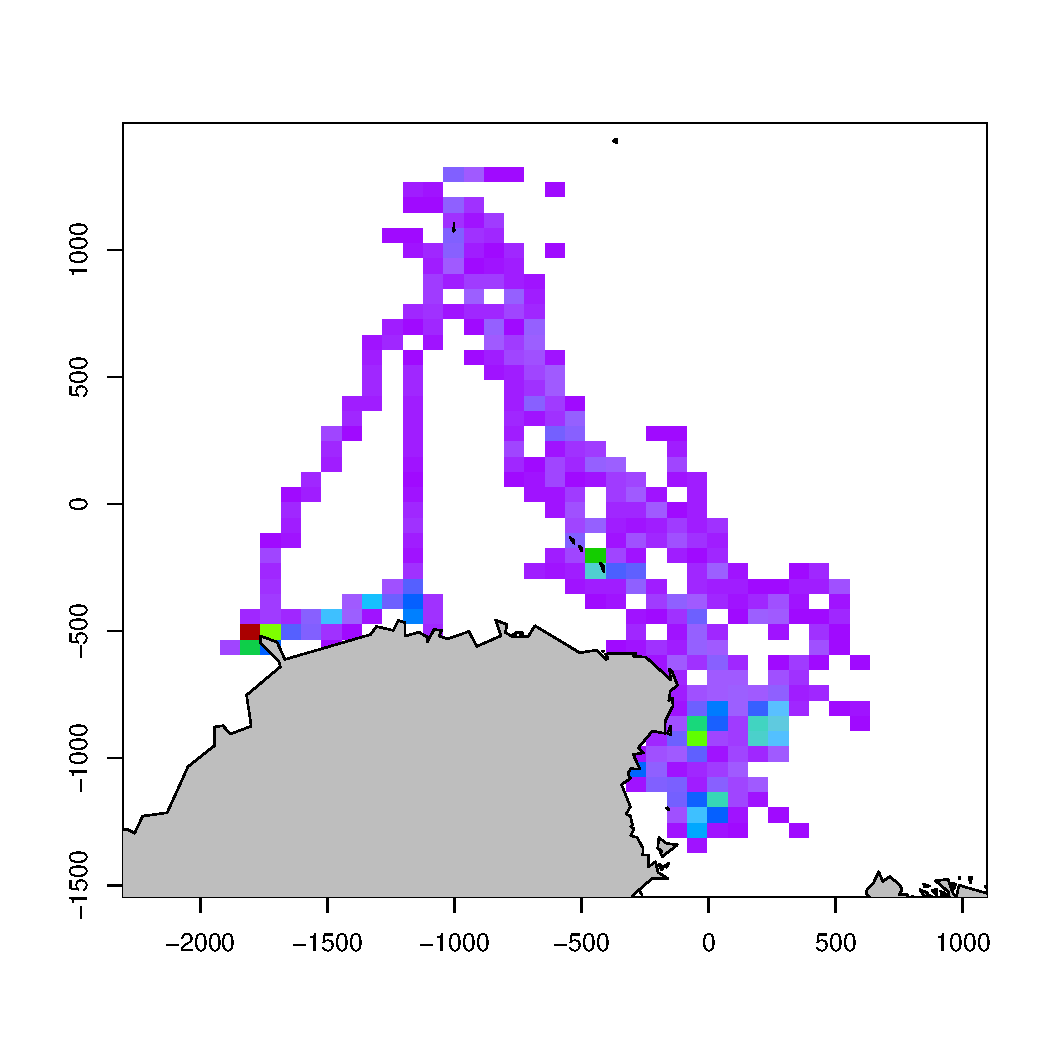
\includegraphics[width=\maxwidth]{figure/minimal-unnamed-chunk-40-1} 

}



\end{knitrout}
\end{center}
\caption{A relatively coarse version of \texttt{fourgrids} with a
  specific kilometre-based cell size (80x60km), specified within an
  equal area map projection.}
\label{fig:coarsegrid}
\end{figure}

%% clip(usr[1], usr[2], usr[3], usr[4])

The first example shows the creation of a grid topology with
dimensions of 50x50, then another is created using cell size. The
resulting plot from this coarser version in an equal area map
projection is shown in Figure~\ref{fig:coarsegrid}. The grid
generation will assume kilometres for cell size as at the centre of
the grid for longitude and latitude coordinates.

For approximate methods \texttt{tripGrid.interp} will interpolate
between positions based on a specified time duration.  A shorter
period will result in a closer approximation to the total time spent,
but will take longer to complete. The approximate method is similar to
that published by \cite{Taylor:BIRD} and \cite{BHMS02}.

% %% Funky animation?
% %% lapply(split(tr, cut(tr$gmt, "1 days")),
% function(x) {plot(x, xlim = bbox(tr)[1,], ylim = bbox(tr)[2,]);
%   degAxis(1);degAxis(2);
%   box();lines(x);
%   map(add = TRUE);
%   Sys.sleep(0.2);NULL})

% \subsection{Integration with GIS}
% Export results above to GeoTIFF.

% Export trips to shapefile / MapInfo format as points or lines.

% Point out limitations of line/point interpretation in GIS.

\section{The need for a more general framework}
Previous sections presented tools for a more systematic handling of
animal track data and a variety of methods for improving track
estimates and deriving spatial summaries such as time spent. Some of
the problems with animal tracking are relatively simple and have
reasonable solutions. The traditional methods above illustrate ways of
dealing with them in an extensible software toolkit. Most of these
solutions however are just ``single-targets''---the easiest aspects are
cherry-picked for a first-pass answer that solves a small aspect of
the larger problem.

Location estimates from methods such as archival tagging and acoustic
tagging can also be dealt with in this way, and there are many studies
that apply these techniques as well as more sophisticated
models. There is an important opportunity here though since the normal
``data product'' for archival tags is not location estimates over time
but dense temporal records of environmental values, such as light,
temperature and depth.

Importantly, different satellite methods such as the Argos Service and
GPS will be handled uniformly by a general approach. These methods
ultimately rely on data as raw as archival tags and acoustic arrays,
with doppler shifts or ephemeris data used to determine location. The
practical difference of these methods from those of archival tags is that
the raw data are simply not available for research purposes, for a
variety of reasons.

% In terms of the data presented, these are locations derived from raw
% data that the researcher has little or no ability to modify. Argos
% publish estimates with simple error categories and techniques for
% light level geolocation can be complicated, with few existing tools
% for carrying them out.

% Considering light level geolocation as a method involving raw sensor
% data, there are issues of inherent accuracy, with the need to process
% light measurements for attenuation, potential cloud cover, dependence
% on paired twilights and equinox problems. The same issues with accuracy
% exist for Argos methods, but the researcher has no control over them
% so the estimation is effectively a black box ['Same?' what does that
% mean, what is the same, similar, etc. - other issues that similarly
% lead to inaccuracies].

% Part of the problem comes from the diversity of needs for different
% researchers and a resulting lack of consistency in approaches.

%% Include stuff about the vagaries of different tags: Argos position
%% classes, archival tag processing, Argos use of speed pre-processing


Another great opportunity presented by raw data is that the concept of
integration of all data sources comes very naturally. For example,
determining position by light level is plagued by environmental
conditions that attenuate the ambient light, and the movement of
animals complicates the relation of environmental measurements to
independent data sets. The scale of measurement is another issue when
relating values such as dive depth or water temperature to synoptic
data sets.

To turn attention to ``raw data'' methods such as those required for
archival tags, the aim is to provide a more complete solution that
integrates solar information, environmental values such as temperature
and depth and applies constraints on movement. This approach contrasts
with the filters in this chapter by applying as much information to
each location estimate as possible. Also it aims to prevent the
practice of discarding ``bad'' location estimates data---the influence
of unreliable data should be downplayed but not ignored completely.

There are of course many existing location estimates for which
there is no rawer data. From this perspective an Argos location can be
treated as a mere data point---not an absolute position to be retained
or discarded and then smoothed by some mechanism, but simply a piece
of data to help inform our models. Even completely invalid positions
have a date-time value and so at the very least it can be inferred
that the animal was ``visible'' to the remote sensing system. In
conjunction with other data about the environment this tiny piece of
data can be valuable.

The following describes the problems specific to the two types of tags that
originally motivated this work. By considering the location estimates
that come from archival tag methods we see that dealing with the
points without reference to the other available information is not
going to be good enough.

\subsection{Location estimation from raw archival data}
Earlier methods of light level geo-location rely on the determination
of critical times during the day from the sequence of raw light
levels.  Longitude is determined directly from the time of local noon
which, based on the symmetry between dawn and dusk, can be easily
measured. Latitude is determined by the length of the day, measured by
choosing representative times such as dawn or dusk that are
distinctive in the light record. While this is a very simplified
explanation given the range of traditional methods the thrust of the
argument is basically correct, see Chapter~\ref{chapter3} and
\cite{M01} for more detail.

In effect, this approach reduces the data set of light values to a
more abstract summary with local peaks at noon and inflection points at
dawn and dusk. The majority of the light data is not used directly and
only one location can be determined per day. This approach to
estimation is susceptible to the movement of the animal between
twilights, to poor choices for the critical times, and to day length
at equinox periods. \cite{HB01}, \cite{Ekstrom} and \cite{Welch1999}
review these methods and provide quantifications for their accuracy.

There is an opportunity for delving more deeply into the raw data
available for location estimation provided by archival
tags. Considering the problems for quality testing of derived
locations, studies can utilize the raw data from the archival tag
and provide an estimation that takes into account more information
such as the conditions at twilight, diving depth, water temperature,
and movement in an integrated way. The raw data is not just a single
point estimate to be discarded or corrected, but a sequence of light,
a sequence of temperature and a sequence of depths. These are all
linked temporally within the main data set. In theory, this is no
different for satellite tags except in that case the raw data are not
available. Raw data in this case would be the doppler shift signals
and satellite orbital details for Argos, and satellite ephemeris and
signal timings for GPS. Acoustic tagging applications similarly have a
wealth of raw data for informing locations, and potential for
improving on existing techniques.

Figure~\ref{fig:refGunn} presents another example of the ``obvious''
problem, with archival tracks that are very erratic and have some
estimates well inland. The sorts of inaccuracies shown tend to be
easily understood by researchers, but the public perception of
research, so important to biological programs, can be easily
undermined by figures like this. This figure also highlights the need
for uncertainty in estimates to be integrated and represented as part
of track visualizations and other summaries.

\begin{figure}[!ht]
  \begin{center}
 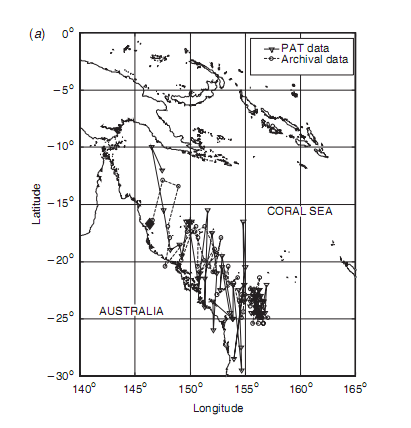
\includegraphics[width=120mm]{roughfigures/gunnArchival.png}
  \end{center}
  \caption{ Light level geo-locations for black marlin in the Coral
    Sea. This image is taken from Figure~3a in \cite{Gunn:GEOL} and is
    reproduced with the permission of the authors.  }
  \label{fig:refGunn}
\end{figure}

\subsection{Filtering locations}

Destructive filters that remove ``erroneous'' locations are
susceptible to the following problems. Data is lost, and this may be
significant for a diving animal or other situation where the
opportunity for obtaining fixes is rare as was shown earlier in
Section~\ref{sec:destructivefilter}. If nothing else, an ``erroneous''
location at least has useful information about the time at which a fix
was available. In practice techniques tend to smooth out some filter
metric across multiple locations, with no clear reason to choose one
technique over another. Speed, distance and direction all require at
least two locations for their calculation, and so this forces the
consideration of a point or line interpretation, or perhaps a hybrid
of the two. The removal of a data point changes the relevant filter
decision for its neighbours and so begs the question of whether the
first location removed is not more valid, and perhaps better than
others that should be removed in preference. An example of this can be
seen with Argos diagnostic (DIAG) data in which there are paired
solutions for each locations \citep{Argos:MAN}. Usually the choice is
obvious, but for many positions it depends on the choice made for
neighbouring locations.  Updating a location to an estimate nearer its
neighbours based on some constraint may be more sensible as in
Section~\ref{sec:penalty}, but there is still only a point
estimate. Preferably there should be a probability distribution for
the location, something that gives an indication of ``how correct''.

\subsection{Intermediate locations}
There is a need for modelling the location of the animal at times that
are not accompanied by data. As discussed in
Section~\ref{sec:surfaces} the goals of cell gridding and density
analysis attempt to integrate this with location uncertainty, but
there are limits to the use of tracks represented by simple points and
lines. In Chapter~\ref{chapter3} an approach that distinguishes
``primary'' locations from ``intermediate'' locations is
presented. The importance of this for track representations is
illustrated in greater detail in Chapter~\ref{chapter5}.

%\subsection{A Bayesian approach}


\section{Conclusion}
This chapter has presented traditional solutions to many of the issues
faced by tracking analyses with a readily available and extensible
software toolkit. The \pkg{trip} package developed by the author
provides an integrated environment for applying traditional algorithms
in the context of widely used spatial data tools. Seemingly isolated
problems with track data were shown to be inter-related in complicated
ways that preclude an otherwise simple chaining together of individual
solutions. The scope of these problems can be extended to include
archival tag data and raw methods like light level geo-location. This
highlights the need for treating any data, even ostensibly accurate
location estimates, as only part of a larger suite of available
information. The next chapter provides an integrated statistical
approach to modelling location using these disparate types of tag
data.



% Add in the bibliography
% Set the text size to be small
\small
% Set the bibliography style

%% relies on apalike.bst, natbib.bst, natbib.sty
\bibliographystyle{apalike}
% List all citations in thesis.bib file
% Comment this out for final printing
% if you have un-cited items in your
% bib database
%\nocite{*}
% thesis.bib is the name of our database
% and we load it with the following command
%\bibliography{mdsRefs}

\end{document}








